%
% Positronium-hydrogen Kohn variational method scattering paper
%

%\documentclass[preprint,showpacs,showkeys,preprintnumbers,amsmath,amssymb,longbibliography,pra,aps,superscriptaddress]{revtex4-1}
\documentclass[preprint,showpacs,showkeys,preprintnumbers,amsmath,amssymb,longbibliography,pra,aps]{revtex4-1}
%\documentclass[reprint,showpacs,preprintnumbers,amsmath,amssymb,pra,aps,longbibliography]{revtex4-1}

% Denton's shortcuts
\newcommand{\ee} {\,\text{e}}
\newcommand{\ii}{{\rm{i}}}

% Packages

\usepackage{graphicx}  % Include figure files
%\usepackage[draft]{graphicx}  % Do not include figure files
\usepackage{dcolumn} % Align table columns on decimal point
\usepackage{bm} % bold math
\usepackage{float}  % @TODO: Take this out before submission!
\usepackage{todonotes}
\usepackage[hidelinks]{hyperref}  % For clickable references
\usepackage{amssymb}
\usepackage{xcolor}
\usepackage{wasysym}  % Simply for \CIRCLE and \Circle (could use \circ for the latter)
\usepackage{subfig}

\usepackage{silence}
\WarningFilter{revtex4-1}{Repair the float}  % Completely innocuous warning - http://tex.stackexchange.com/questions/180762/revtex4-1-warning-repair-the-float-package

% Subfolders containing our images
\graphicspath{{IPython/}{Images/}}

% To center table head
\newcommand*{\thead}[1]{\multicolumn{1}{c}{#1}}

\setlength{\abovecaptionskip}{0pt}  % Reduce space between figure and caption (default of 10pt)
\setlength{\paperheight}{11in}  % To get rid of the annoying hyperref warning


\begin{document}

%\preprint{APS/123-QED}

\title{A Detailed Investigation of Low-Energy Positronium-Hydrogen Scattering}

\author{Denton Woods}
\email{denton.woods@unt.edu}
\homepage{http://www.dentonwoods.com}

\author{S. J. Ward}
\affiliation{Department of Physics, University of North Texas, Denton, Texas 
76203, USA}

\author{P. Van Reeth}
\affiliation{Department of Physics and Astronomy, University College London, 
Gower Street, London WC1E 6BT, UK}

\date{\today}

\begin{abstract}
We investigate the four-body Coulomb process of low-energy elastic
positronium-hydrogen (Ps-H) scattering below the Ps(n=2) excitation threshold
using scattering wavefunctions that include Hylleraas-type 
correlation terms. Using the complex Kohn variational method, we 
compute phase shifts through the $^{1,3}H$-wave and obtain highly accurate
$^{1,3}S$- and $^{1,3}P$-wave phase shifts. The complex
Kohn variational results compare well to a number of other calculations for 
this system. In addition, we present elastic 
differential, elastic integrated, and momentum transfer
cross sections, and for the singlet, resonances through the
$^1F$-wave. The differential cross section exhibits interesting features,
including a change from slightly backward peaked to
forward peaked scattering as the energy of the incident
positronium increases and
rich structure due to multiple resonances near the Ps(n=2) threshold.
We also give a detailed analysis of the scattering lengths
and effective ranges using multiple effective range theories.
\end{abstract}

   
\pacs{31.15.xt Variational techniques; 34.50.-s Scattering of atoms and
molecules; 36.10.Dr Positronium; 34.80.Bm Elastic scattering}
\keywords{positronium; PsH; positronium hydride; Kohn variational}
\maketitle

\section{\label{sec:Intro}\protect Introduction}


%\preprint{APS/123-QED}

Positronium (Ps) scattering from atoms and molecules is an area of current 
experimental and theoretical interest. The development of energy-tunable
ortho-Ps beams
\cite{Brown1985,Laricchia1987,Zafar1996,Garner1996,Laricchia2008} 
has enabled measurements to be made of Ps scattering from the inert gases He,
Ne, Ar, Kr, and Xe
\cite{Garner1996,Garner2000,Armitage2002,Laricchia2004,Armitage2006,Laricchia2008,Engbrecht2008,Brawley2010a}
and the molecules H$_2$, N$_2$, O$_2$, CO$_2$, H$_2$O, and SF$_6$
\cite{Garner1996,Garner1998,Garner2000,Laricchia2004,Armitage2006,Beale2006,Brawley2010a}.
Cross sections for Ps scattering from H have not been measured due to the
difficulty of creating an H beam, although the binding energy of positronium
hydride (PsH) has been measured in the reaction of a positron with methane,
e$^+$ + CH$_4$ $\to$ CH$_3^+$ + PsH \cite{Schrader1992}. The low-energy region
is of particular interest, because in this energy range, positron and electron 
correlations are important. We present
our work of the application of the complex Kohn variational 
method to elastic Ps(1s)-H(1s) scattering for the energy range
up to the excitation threshold of Ps(n=2) at $\tfrac{3}{16}$ a.u.
(5.102 eV) \cite{Conferences1,Conferences2,Conferences3,WoodsDiss2015}.

Ps-H scattering is a fundamental four-body Coulomb process. The Kohn and 
inverse Kohn variational methods have previously been applied to Ps-H 
collisions by Van Reeth and Humberston \cite{VanReeth2003,VanReeth2004}, who 
computed $^{1,3}S$ and $^{1,3}P$ phase shifts. We 
extend their $^{1,3}S$ and $^{1,3}P$  variational calculations in 
multiple ways. In addition to
the Kohn and inverse Kohn variational methods, we implement the 
generalized Kohn method, and the complex Kohn methods for the $S$ and $T$ matrices.
The complex Kohn methods for the $S$ and $T$ matrices
are known to suffer from far fewer anomalous singularities than the Kohn,
inverse Kohn and generalized Kohn variational methods
\cite{Lucchese1989, Cooper2009, Cooper2010}. Another extension that we
consider is to use the procedure by Todd 
\cite{Todd2007} to systematically remove short-range terms that cause linear 
dependence. This enables us to compute the phase shifts
with more short-range Hylleraas terms than the earlier 
Kohn and inverse Kohn variational calculations
\cite{VanReeth2003, VanReeth2004}.
We add the asymptotic expansion of Drake and Yan
\cite{Drake1995, Yan1997} to improve the accuracy of matrix elements
containing only short-range terms. We significantly increase
the number of integration points for matrix
elements that involve the long-range terms, along with implementing a
procedure to
accelerate the convergence of these integrals (introduction
and subsequent removal of exponential terms to the Gauss-Laguerre
quadratures). We also extend the 
calculations to the next four partial waves through to the $H$-wave, which
enables us to calculate the elastic differential, elastic integrated,
and momentum transfer cross sections.

We present results in this paper obtained generally using the $S$-matrix
complex Kohn 
variational principle for Ps-H scattering. We confirm the previously calculated 
resonances for the first four partial waves and compare the resonance parameters
to those of the earlier Kohn \cite{VanReeth2004}, close 
coupling (CC) \cite{Walters2004} and complex rotation calculations
\cite{Yan1999,Yan1998a,Ho1998,Ho2000}. In addition, we compute the scattering
lengths and effective ranges using multiple effective range theories.

We use the short-range part of the full scattering wavefunction to 
compute the binding energy of PsH. The binding energy
of PsH, $E_b$, has been calculated using various methods. Ho \cite{Ho1986}
performed a variational calculation with a Hylleraas-type basis set, and Yan and Ho
\cite{Yan1999} later did a more extensive calculation. Mitroy \cite{Mitroy2006}
used the stochastic variational method (SVM) with 1800 explicitly correlated 
Gaussians (ECGs), and Bubin and Adamowicz \cite{Bubin2006} found the most 
accurate value to date using 5000 ECGs in a variational calculation.

There have been a number of other calculations for Ps-H scattering. A much 
earlier Kohn variational calculation was performed by Page \cite{Page1976} 
for the Ps-H scattering lengths. Drachman and Houston
\cite{Drachman1975,Drachman1976} used
a stabilization method with an effective range theory (ERT) expansion.
At low energies, diffusion Monte Carlo (DMC)
\cite{Chiesa2002}, the SVM \cite{Ivanov2001,Ivanov2002}, CC
\cite{Sinha1997,Campbell1998,Adhikari1999,Sinha2000,Blackwood2002,Blackwood2002b,Walters2004},
static exchange \cite{Hara1975,Ray1997,*Ray1996}, Kohn variational
\cite{Page1976,VanReeth2003,VanReeth2004}, and inverse Kohn
variational \cite{VanReeth2003,VanReeth2004} methods have been applied. The SVM
with stabilization 
techniques was used to compute low-energy phase shifts and 
scattering lengths for Ps-H collisions \cite{Ivanov2001,Ivanov2002}.

The first Born approximation has been used by Massey and Mohr \cite{Massey1954}
and later by McAlinden et al.~\cite{McAlinden1996}.
Blackwood et al.~\cite{Blackwood2002} performed an elaborate CC calculation 
for Ps scattering from H, which took into account excitation and ionization 
of both the projectile and target. They considered two different coupling 
schemes. The first one, which they refer to as 9Ps9H, included 9 eigen- and 
pseudo-states of Ps and also of H. The second scheme, which they refer to as 
14Ps14H, was used for $S$-wave singlet scattering only and included
14 eigen- and pseudo-states of 
Ps and also of H. Good agreement was obtained between the CC
\cite{Blackwood2002} and the SVM \cite{Ivanov2002} for the $^{1,3}S$-wave scattering
lengths and phase shifts. In another paper, Blackwood et
al.~\cite{Blackwood2002b} considered the importance of including the H$^-$
channel in a 22Ps1H coupling scheme, comparing with the previous 22Ps1H
calculations of Campbell et al. \cite{Campbell1998}. Walters et
al.~\cite{Walters2004} extended the earlier CC calculations
\cite{Blackwood2002} to include the e$^+$-H$^-$ channel
\cite{Blackwood2002b} and compared their results for the $S$-wave with the
Kohn variational results \cite{VanReeth2003}.
A recent calculation of Ps-H scattering by Zhang and Yan
\cite{Zhang2012} used the
confined variational method (CVM) to calculate phase shifts for two momenta
for both $^1S$ and $^3S$. This method provides accurate
results but has the drawback of being very computationally expensive.

The Kohn variational method gives rigorous upper bounds on the scattering lengths
and, except for Schwartz singularities, empirical lower bounds on the
phase shifts. This means that the wave 
function can be systematically improved to the converged results. The Kohn 
and inverse Kohn
variational methods are known to yield accurate results and have provided 
benchmark results \cite{VanReeth2003,VanReeth2004} with which results from 
other calculations can be compared.

Phase shifts are expressed in radians. Atomic units are used throughout 
unless otherwise stated. For conversions to electron-volts (eV), we use the 
conversion factor 1 a.u. = {27.21138505(60) eV}
\cite{Mohr2012,*NISTConversions}.

%\emph{Add \cite{Shipman2014}, \cite{Barker2012}, \cite{Laricchia2009}?}
%\emph{Add \cite{Mitroy2002a}?}


\vskip 0.5truecm
\noindent
\section{Theory}

\subsection{The Positronium-Hydrogen System and Trial Scattering Wavefunctions}
\begin{figure}[H]
	\centering
	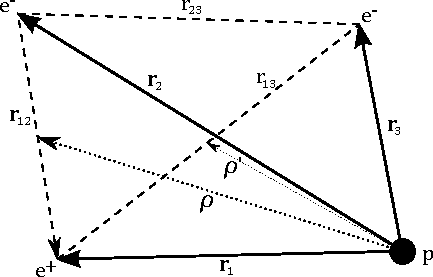
\includegraphics[height=2in]{PsHCoordinates}
	\caption{Positronium-hydrogen coordinate system}
	\label{fig:PsHCoords}
\end{figure}

We investigate low-energy elastic scattering of ground-state Ps
with ground-state H, Ps(1s)+H(1s), for incident energies up to the excitation
threshold of Ps(n=2).
Previous work on Ps-H scattering used the Kohn and inverse Kohn variational
methods \cite{VanReeth2003, VanReeth2004}. 
Van Reeth and Humberston \cite{VanReeth1999} used the complex Kohn 
variational method for e$^+$-He scattering. While we generally present
results in Sec. \ref{sec:Results} that we obtain using the $S$-matrix
complex Kohn variational method, here we present in
this section a general wavefunction that can be used in the Kohn
variational method and a number of its variants,
as we describe in Sec.~\ref{sec:Kohn}.

For $S$-wave Ps(1s)-H(1s) elastic scattering, the flexible scattering
wavefunction is given by
\begin{equation}
\Psi_0^{\pm,t} = \widetilde{S}_0 + L_0^{\pm,t} \, \widetilde{C}_0
  + \sum_{i=1}^{N(\omega)} c_{i0} \bar{\phi}_{i\ell 1},
\label{eq:TrialWave}
\end{equation}
where the superscript $t$ indicates that this is a trial wavefunction. The plus
sign indicates the spatially symmetric singlet case, and the minus sign
indicates the spatially antisymmetric triplet case. The total orbital angular
momentum of the system is equal to the orbital angular momentum $\ell$ 
of the incoming Ps(1s). For partial waves $\ell > 0$, we consider a trial
wavefunction of the form
\begin{equation}
\Psi_\ell^{\pm,t} = \widetilde{S}_\ell + L^{\pm,t}_\ell \, \widetilde{C}_\ell
 + \sum_{i=1}^{N(\omega)} c_{i\ell} \bar{\phi}_{i\ell 1}
 + \!\!\!\sum_{i=N(\omega)+1}^{2N(\omega)} \!\! d_{i\ell} \bar{\phi}_{i\ell 2}.
\label{eq:TrialWaveHigher}
\end{equation}
The scattering wavefunctions contain both the long-range terms $\widetilde{S}_\ell$
and $\widetilde{C}_\ell$ and the short-range terms $\bar{\phi}_{i\ell k}$. The 
long-range terms of Eqs. (\ref{eq:TrialWave}) and (\ref{eq:TrialWaveHigher})
are given by
\begin{equation}
\label{eq:SCPhiDef}
\begin{bmatrix}
\widetilde{S}_\ell \\ \widetilde{C}_\ell
\end{bmatrix} = \textbf{u}  \begin{bmatrix}
\bar{S}_\ell \\ \bar{C}_\ell
\end{bmatrix} = \begin{bmatrix}
u_{00} & u_{01} \\  u_{10} & u_{11}
\end{bmatrix}
\begin{bmatrix}
\bar{S}_\ell \\ \bar{C}_\ell
\end{bmatrix}, 
\end{equation}
where
\begin{equation}
\label{eq:SBar}
\bar{S}_\ell = \frac{1\pm P_{23}}{\sqrt{2}}Y_{\ell 0}(\theta_\rho,
  \varphi_\rho)\Phi_{{\rm{Ps}}(1s)}\!\left(r_{12}\right) \Phi_{{\rm{H}}(1s)}\!\left(r_3\right)
  \sqrt{2\kappa} \,j_\ell\left(\kappa\rho\right)
\end{equation}
and
\begin{equation}
\label{eq:CBar}
\bar{C}_\ell = -\frac{1\pm P_{23}}{\sqrt{2}}Y_{\ell 0}(\theta_\rho,
  \varphi_\rho)\Phi_{{\rm{Ps}}(1s)}\!\left(r_{12}\right) \Phi_{{\rm{H}}(1s)}\!\left(r_3\right)
  \sqrt{2\kappa} \,n_\ell\left(\kappa\rho\right) f_\ell(\rho).
\end{equation}
Fig.~\ref{fig:PsHCoords} gives the
coordinate system for Ps-H. The vector
$\bm{\rho} = \frac{1}{2}\left(\bm{r_1} + \bm{r_2}\right)$ is the position
vector of the center of mass of the Ps atom with respect to the proton,
$j_\ell\left(\kappa\rho\right)$ and $n_\ell\left(\kappa\rho\right)$ are
the spherical Bessel and Neumann functions respectively, and
$Y_{\ell m}(\theta_\rho, \varphi_\rho)$ is the spherical harmonic for $m = 0$.
$P_{23}$ is the exchange operator for the two indistinguishable electrons, and
$\Phi_{{\rm{Ps}}(1s)}\!\left(r_{12}\right)$ and
$\Phi_{{\rm{H}}(1s)}\!\left(r_3\right)$ are the ground-state wavefunctions
of Ps and H, respectively. The shielding factor, $f_\ell(\rho)$,
removes the singularity of the spherical Neumann function
at the origin. We choose it to have the form
\begin{equation}
f_\ell(\rho) = \left[1 - \ee^{-\mu \rho} \left(1+\frac{\mu}{2}\rho\right)
\right]^{m_\ell}.
\label{eq:PartialWaveShielding}
\end{equation}
Table \ref{tab:Nonlinear} shows the values of the
nonlinear parameter $\mu$ and the integer $m_\ell$ we use for each partial
wave.

We consider the Kohn variational method and a number of its variants,
and $\textbf{u}$ and $L^{\pm}_\ell$ take
different forms depending on which one:
\begin{subequations}
\label{eq:KohnU}
\begin{align}
&\text{generalized Kohn, } L^{\pm,t}_\ell = \tan(\delta^{\pm,t}_\ell-\tau),
 \textbf{u} = \left[ \begin{smallmatrix}
\cos \tau & \ \sin \tau \\  -\sin \tau & \  \cos \tau
\end{smallmatrix} \right], \label{eq:GenKohn}\\
&\text{generalized $T$-matrix complex Kohn, } L^{\pm,t}_\ell = T_\ell^{\pm},
 \textbf{u} = \left[ \begin{smallmatrix}
\cos\tau & \ \sin\tau \\ -\sin\tau + \ii \cos\tau & \ \cos\tau + \ii \sin\tau
\end{smallmatrix} \right] \label{eq:GenTKohn} \\
&\text{generalized $S$-matrix complex Kohn, } L^{\pm,t}_\ell = -S_\ell^{\pm},
 \textbf{u} = \left[ \begin{smallmatrix}
-\ii \cos\tau - \sin\tau & \ -\ii\sin\tau + \cos\tau \\ 
 \ii\cos\tau - \sin\tau & \ \ii\sin\tau + \cos\tau
\end{smallmatrix} \right]. \label{eq:GenSKohn}
\end{align}
\end{subequations}
For the case of $\tau = 0$, these give the Kohn, the $T$-matrix and
$S$-matrix complex Kohn variational methods, respectively.
$\tau = \frac{\pi}{2}$ in Eq. (\ref{eq:GenKohn})
gives the inverse Kohn. 
For comparison with Cooper et al.\ \cite{Cooper2010}, the generalized
Kohn \textbf{u} matrix is identical to their corresponding matrix,
while the \textbf{u} matrix for the generalized $T$-matrix complex Kohn
is similar to their corresponding matrix.
We use the definition of the $T$ and $S$ matrices
given by Bransden \cite{Bransden1970}.
The \textbf{u} matrix for the Kohn in Eq.~(\ref{eq:KohnU}) is identical
to that of Lucchese \cite{Lucchese1989}, but the \textbf{u} matrices for
the inverse Kohn, $T$ matrix, and $S$ matrix are slightly different.

The short-range terms are highly correlated Hylleraas-type functions, including
all interparticle distances, given by
\begin{align}
\label{eq:PhiDef}
\bar{\phi}_{i\ell k} = &\left(1 \pm P_{23}\right) Y_{\ell 0}(\theta_k,\phi_k)
e^{-(\alpha r_1 + \beta r_2 + \gamma r_3)} \nonumber \\
&\times r_k^{\ell} r_1^{k_i} r_2^{l_i} r_{12}^{m_i} r_3^{n_i} r_{13}^{p_i} r_{23}^{q_i}.
\end{align}
The variable $\omega$ is a non-negative integer that determines the maximum
number of terms in the basis set. For a chosen value of $\omega$, the integer
powers of $r_i$ and $r_{ij}$ are constructed in such a way that 
\begin{equation}
k_i + l_i + m_i + n_i + p_i + q_i \leq \omega,
\end{equation}
with all $k_i, l_i, m_i, n_i, q_i$ and $p_i \geq 0$ \cite{VanReeth2004}.
The first set of short-range terms in Eq. (\ref{eq:TrialWaveHigher}), which we
refer to as the first symmetry, has $k=1$ for $i=1$ to $N(\omega)$. The second
symmetry set of terms exists for $\ell > 0$, with $k=2$ and $i = N(\omega)+1$
to $2N(\omega)$. These short-range terms represent the angular momentum as
being placed on either the positron ($r_1$) or on the electron {in the Ps
atom ($r_2$, and $r_3$
with exchange). Following up on Ref. \cite{VanReeth2004} where the slow 
convergence of the $^3P$ phase shift was discussed, we also consider a 
wavefunction where the angular momentum was placed on the electron of the H 
atom ($r_3$) and on the Ps ($\rho$). Since we find that this did not improve the
accuracy of the results, and in some cases, the phase shifts seem less
accurate, we do not present results from this alternative
formalism here.
In Sec.~\ref{sec:Numerical}, we discuss numerical techniques that improve
convergence of the results.

For partial waves with $\ell>1$, the orbital angular momentum could also be 
shared between both particles in the Ps atom, giving a total of
$\ell + 1$ sets of short-range terms \cite{Schwartz1961a}. For the
$D$-wave, this gives another set of short-range terms in
Eq.~(\ref{eq:TrialWaveHigher})
\cite{Humberston1997,VanReethThesis,BrownThesis}, referred to as the mixed
symmetry terms, which were included for the three-body system of e$^+$-H
in earlier work of
Refs.~\cite{Brown1985a,BrownThesis,WattsThesis,Humberston1997,VanReeth1997}.
Van Reeth and Humberston \cite{VanReeth1997} found that these
mixed symmetry terms contributed less than 1.5\% to the $K$ matrix elements
for e$^+$-H scattering, but this result now appears to be in error.
A preliminary investigation for e$^+$-H \cite{VanReeth2015} with a corrected
code has shown 
that these mixed symmetry terms can be important for that 
system. This investigation found that
including the mixed symmetry terms changes
the phase shifts by less than 1\% at $\kappa = 0.1$, and near the Ps formation
threshold, by about 10\%. Fortunately, in the earlier $D$-wave e$^+$-H
scattering
calculation \cite{Humberston1997}, the inclusion of the virtual Ps terms
represented sufficiently well the required spatial configuration so that it
compensated for the lack of convergence due to the
error in the previous inclusion of the mixed symmetry
terms. The final numerical results used in Ref. \cite{VanReeth1997} are
within 1 to 2\% of the phase shifts of the preliminary
calculation \cite{VanReeth2015} that correctly
includes the mixed symmetry terms and for which the virtual Ps terms have
been found to make no significant contribution. The investigation of
Ref.~\cite{VanReeth2015} has been extended to
e$^-$-H scattering, and it has revealed that
for the $^1D$-wave, the inclusion of the 
mixed symmetry terms has little effect on the phase shifts at very low
energies but has a more appreciable effect at higher energy. Interestingly,
this investigation found that the mixed symmetry terms change the
$^3D$-wave e$^-$-H phase shifts less than 1\% over the energy
range considered.

As discussed in Sec.~\ref{sec:Results} for Ps-H scattering, the $D$-wave
contributes only a small amount to the elastic integrated cross sections away 
from the $^1D$ resonance. Therefore, due to the complexity of the analytical 
forms for the four-body system, we do not explicitly include the mixed 
symmetry terms for Ps-H scattering.


% THE HAMILTONIAN
The Hamiltonian for the Ps-H system is
\begin{align}
H = -&\frac{1}{2} \nabla_{r_1}^2 - \frac{1}{2} \nabla_{r_2}^2 - \frac{1}{2}
  \nabla_{r_3}^2  \nonumber \\
&+ \frac{1}{r_1} - \frac{1}{r_2} - \frac{1}{r_3} - \frac{1}{r_{12}} -
  \frac{1}{r_{13}}+\frac {1}{r_{23}},
\label{eq:Hamiltonian1}
\end{align}
which, using Jacobi coordinates for the kinetic energy operator, can be
expressed as
\begin{align}
H = -&\frac{1}{4} \nabla_{\rho}^2 - \frac{1}{2} \nabla_{r_3}^2 -
  \nabla_{r_{12}}^2  \nonumber \\
&+ \frac{1}{r_1} - \frac{1}{r_2} - \frac{1}{r_3} - \frac{1}{r_{12}} -
  \frac{1}{r_{13}}+\frac{1}{r_{23}}.
\label{eq:Hamiltonian2}
\end{align}


\subsection{Derivation of the Kohn Variational Method and Variants of the Method}
\label{sec:Kohn}
The derivation we present here for the Kohn variational method and its variants
follows a similar procedure given in
Refs.~\cite{Lucchese1989,Cooper2010,Armour1991,VanReethThesis}.
The functional for the full wavefunction in Eqs. (\ref{eq:TrialWave}) and
(\ref{eq:TrialWaveHigher}) is (dropping the $\ell$ subscript and the $\pm$ 
superscript for brevity),

\begin{equation}
I[\Psi^t] = \left(\Psi^t, \mathcal{L} \Psi^t \right) = \int \Psi^t \mathcal{L}
  \Psi^t \,d\tau,
\label{eq:IlDefPsi}
\end{equation}
with
\begin{equation}
\mathcal{L} = 2(H - E).
\label{eq:LDef}
\end{equation}
The total energy of the system, $E$, is given by
\begin{equation}
\label{eq:TotalEnergy}
E = E_H + E_{Ps} + \frac{1}{4}\kappa^2 = E_H + E_{Ps} + E_{\bm \kappa},
\end{equation}
where $E_H$ and $E_{Ps}$ are the ground-state energies of H and Ps, 
respectively,
and $E_{\bm \kappa}$ is the kinetic energy of the incoming Ps atom.
The complex conjugate of $\Psi^t$ that premultiplies $\mathcal{L} \Psi^t$
is not taken for a consistent derivation of the complex Kohn variational
methods \cite{Cooper2010,Lucchese1989}.

We assume the trial wavefunction $\Psi^t$ is a small variation of the exact
wavefunction
$\Psi$, or
\begin{equation}
\Psi^t = \Psi + \delta \Psi.
\label{eq:PsiTrialRelation}
\end{equation}
It can be shown that the variation in the functional $I$,
$\delta I = I[\Psi^t] - I[\Psi] = I[\Psi^t]$,
is given by
\begin{equation}
\delta I = (L^t - L) \det \textbf{u} + I[\delta \Psi].
\label{eq:IlPsiVariation}
\end{equation}
Here $L^t$ represents the scattering parameters given by Eq.~(\ref{eq:KohnU})
for the trial wavefunctions given by Eqs.~(\ref{eq:TrialWave}) and
(\ref{eq:TrialWaveHigher}), and $L$ represents the corresponding parameters
(given by Eq.~(\ref{eq:KohnU}) without the `t') for the exact wavefunction.
Neglecting the second-order term in $\delta \Psi$, $I[\delta \Psi]$, and realizing that
$I[\Psi] = 0$, we obtain a functional for the variational $L^v$ of
\begin{equation}
L^v = L^t - I[\Psi^t] / \det \textbf{u}.
\label{eq:ComplexKohnVariation}
\end{equation}

Using the stationary property of the functionals for the Kohn and variants, we obtain
\begin{equation}
\frac{\partial L^v}{\partial L^t} = 0  \text{ and }
  \frac{\partial L^v}{\partial c_i} = 0 \text{ where $i = 1,\ldots,N$},
\label{eq:ComplexKohnStationary}
\end{equation}
which can be written as a matrix equation. For the $S$-wave, the matrix
equation is
\begin{widetext}
\begin{equation}
\label{eq:ComplexKohnMatrix}
\begin{bmatrix} 
 (\widetilde{C},\mathcal{L}\widetilde{C}) & (\widetilde{C},\mathcal{L}\bar{\phi}_{101}) & \cdots & (\widetilde{C},\mathcal{L}\bar{\phi}_{N01})\\
 (\bar{\phi}_{101},\mathcal{L}\widetilde{C}) & (\bar{\phi}_{101},\mathcal{L}\bar{\phi}_{101}) & \cdots & (\bar{\phi}_{101},\mathcal{L}\bar{\phi}_{N01})\\
 \vdots & \vdots & \ddots & \vdots \\
 (\bar{\phi}_{N01},\mathcal{L}\widetilde{C}) & (\bar{\phi}_{N01},\mathcal{L}\bar{\phi}_{101}) & \cdots & (\bar{\phi}_{N01},\mathcal{L}\bar{\phi}_{N01})
\end{bmatrix}
\begin{bmatrix}
L^t\\
c_1\\
\vdots\\
c_N
\end{bmatrix}
= -
\begin{bmatrix}
(\widetilde{C},\mathcal{L}\widetilde{S}) \\
(\bar{\phi}_{101},\mathcal{L}\widetilde{S}) \\
\vdots \\
(\bar{\phi}_{N01},\mathcal{L}\widetilde{S})
\end{bmatrix}.
\end{equation}
\end{widetext}
This matrix equation can be rewritten as
$\textbf{\emph{AX}}$ = -$\textbf{\emph{B}}$, as can the matrix equations
for $\ell > 0$. For higher partial waves,
the matrix equation looks the same but includes the second symmetry
short-range terms and corresponding coefficients. Finally, for arbitrary
$\ell$, we solve for $L^v$,
\begin{equation}
\label{eq:Lv}
L^v = -\frac{1}{\det \textbf{u}} \left( \textbf{\emph{B}}^{tr} \textbf{\emph{X}} +
  (\widetilde{S},\mathcal{L} \widetilde{S}) \right),
\end{equation}
to obtain the phase shifts by using the relation \cite{Lucchese1989}
\begin{equation}
\label{eq:GenKohnL}
K_\ell = \tan \delta_\ell = (u_{01} + u_{11} L_\ell)(u_{00} + u_{10}
  L_\ell)^{-1},
\end{equation}
reintroducing the subscript $\ell$.

\subsection{PsH Bound State}
As done earlier by Van Reeth and Humberston \cite{VanReeth2003,VanReeth2004},
we use the short-range correlation part of the $^1S$-wave scattering wavefunction
to compute the binding energy, $E_b$, of the $^1S$ PsH system. This gives us
some confidence of the reliability of using these short-range terms for the Ps-H 
scattering problem. The wavefunction we use for the bound state is
\begin{equation}
\label{eq:BoundWavefn}
\Psi_{B.S.}^\pm = \sum_{i=1}^{N(\omega)} c_i \bar{\phi}_{i01}^\pm,
\end{equation}
where $\bar{\phi}_{i01}^\pm$ is given in Eq. (\ref{eq:PhiDef}) with
$\ell = 0$.

\subsection{Born-Oppenheimer Approximation}
Using the first term, $\widetilde{S}_\ell$, in the wavefunction,
Eqs. (\ref{eq:TrialWave}) and (\ref{eq:TrialWaveHigher}), for
the Kohn variational method, $\bar S_\ell$, gives for the
Born-Oppenheimer (BO) approximation to $\tan\delta_\ell$ of \cite{Bransden2003}
\begin{equation}
\label{eq:Born}
\tan\delta_\ell^{BO} = -(\bar{S}_\ell,\mathcal{L}\bar{S}_\ell)\,.
\end{equation}
We also consider a modified BO approximation to $\tan\delta_\ell$ that uses
both long-range terms in the wavefunction,
Eqs. (\ref{eq:TrialWave}) and (\ref{eq:TrialWaveHigher}), for the Kohn
variational principle in Eqs. (\ref{eq:Lv}) and (\ref{eq:GenKohnL}).


\subsection{Effective Range Theories}

The scattering length is defined as \cite{Bransden2003}
\begin{equation}
\label{eq:ScatLen}
a_\ell^\pm = -\lim_{\kappa \to 0}
  \frac{\tan{\delta_\ell^\pm}}{\kappa^{2\ell+1}}.
\end{equation}
We consider the approximation with very small $\kappa$ of
\begin{equation}
\label{eq:ScatLenApprox}
a_\ell^\pm \approx
  - \frac{\tan{\delta_\ell^\pm}}{\kappa^{2\ell+1}}.
\end{equation}
To avoid confusion with the Bohr radius, $a_0$, we denote
the $S$-wave scattering length $a_{\ell=0}$ as $a$.

For short-range interactions, the $S$-wave effective range theory (ERT)
expansion is given by \cite{Bethe1949,Blatt1949}
\begin{equation}
\label{eq:EffectiveRangeShort}
\kappa \cot\delta_0^\pm = -\frac{1}{a^\pm} + \frac{1}{2} r_0^\pm \kappa^2,
\end{equation}
where $r_0^\pm$ is the effective range.
This ERT expansion has been used in the literature
\cite{Ivanov2002,VanReeth2003,Blackwood2002,Walters2004} to compute the
scattering length and effective range for Ps-H scattering. 
For the van der Waals (vdW) interaction, which is the dominant long-range
interaction between Ps and H \cite{Fabrikant2014,VanReeth2003,Au1986},
the scattering length is only defined for the $S$- and $P$-waves, and the 
effective range is defined for only the $S$-wave \cite{Levy1963}.
An $S$-wave ERT expansion for the van der Waals interaction is given in
Ref.~\cite{Drake2006}, which for Ps-H scattering where the mass of Ps
is two, has the form
\begin{equation}
\label{eq:EffectiveRangeLongAu}
\kappa \cot\delta_0^\pm = -\frac{1}{a^\pm} + \frac{1}{2} r_0^\pm \kappa^2 - 
  \frac{4 \pi C_6}{15 (a^\pm)^2} \kappa^3 - 
  \frac{16 C_6}{15 a^\pm} \kappa^4 \ln \left(\kappa \right).
\end{equation}
We use the van der Waals coefficient of $C_6 = 34.78473$ a.u., as given
by Martin and Fraser \cite{Martin1980}.

Gao \cite{Gao1998} has developed a quantum defect theory (QDT)
for an attractive $r^{-6}$ potential, obtaining an equation relating
the tangent of the phase shifts to elements of a $Z$ matrix
(see Ref.~\cite{Gao1998}) and an analytic function of energy $K_\ell^0$
\cite{Gao1998a}
\begin{equation}
\label{eq:GaoZEqn}
\tan\delta_\ell = [Z_{ff} - K_\ell^0 Z_{gf}]^{-1}
  [K_\ell^0 Z_{gg} - Z_{fg}].
\end{equation}
$K_\ell^0$ can be expanded in powers of the energy \cite{Gao1998a} of the
incoming Ps atom as
\begin{equation}
\label{eq:GaoKTaylor}
K_\ell^0(E_{\bm \kappa}) = K_\ell^0(0) + {K_\ell^0}^\prime(0) E_{\bm \kappa}
  + \ldots.
\end{equation}
We retain the first two terms in the expansion and determine the coefficients
$K_\ell^0(0)$ and ${K_\ell^0}^\prime(0)$ by fitting the phase shifts to
Eq.~(\ref{eq:GaoKTaylor}). We compute the $^{1,3}S$- and $^{1,3}P$ scattering
lengths and $^{1,3}S$-wave effective ranges using the expressions
given by Gao \cite{Gao1998a}, which relates these quantities to the
coefficients.


\section{Numerics}
\label{sec:Numerical}

We present briefly the numerical techniques below. Details
can be found in Ref.~\cite{WoodsDiss2015}.

\subsection{Short-Short Integrations}
\label{sec:ShortInt}
For the $^1S$ PsH bound state and $^{1,3}S$ Ps(1s)-H(1s) elastic scattering
calculations, we use
the efficient asymptotic expansion method presented by Drake and Yan
\cite{Drake1995} for the evaluation of correlated integrals of the form
\begin{align}
\label{eq:ShortInt}
I(&j_1,j_2,j_3,j_{12},j_{23},j_{31}; \bar{\alpha}, \bar{\beta}, \bar{\gamma}) =
  \nonumber \\
&\int
d \textbf{r}_1 d \textbf{r}_2 d \textbf{r}_3
r_1^{j_1} r_2^{j_2} r_3^{j_3} r_{12}^{j_{12}}
r_{23}^{j_{23}} r_{31}^{j_{31}}
e^{-(\bar{\alpha} r_1 + \bar{\beta} r_2 + \bar{\gamma} r_3)}\, .
\end{align}
These integrals arise from evaluation of the matrix elements
$(\bar{\phi}_{i\ell k}, \mathcal{L} \bar{\phi}_{j\ell k})$,
$(\bar{\phi}_{i\ell k}, H \bar{\phi}_{j\ell k})$,
and $(\bar{\phi}_{i\ell k}, \bar{\phi}_{j\ell k})$, where $H$
is the full Hamiltonian given in Eqs. (\ref{eq:Hamiltonian1}) and
(\ref{eq:Hamiltonian2}).
The relationship between $\bar{\alpha}$ and $\alpha$ can be seen by
considering these matrix elements, as can that of $\bar{\beta}$, $\beta$,
$\bar{\gamma}$, $\gamma$, and the $r_i$ and $r_{ij}$ exponents.
We also use the recursion relations of Pachucki
et al. \cite{Pachucki2004} to confirm the calculations of the short-range 
integrals for the $S$-wave and $P$-wave.

For $\ell > 0$, the short-range integrals have the form of
\begin{widetext}
\begin{align}
\label{eq:ShortIntGen}
\nonumber I(\ell_1^\prime m_1^\prime, \ell_2^\prime m_2^\prime, &\ell_3^\prime m_3^\prime; j_1,j_2,j_3,j_{12},j_{23},j_{31}; \bar{\alpha}, \bar{\beta}, \bar{\gamma}) = \int d \textbf{r}_1 d \textbf{r}_2 d \textbf{r}_3
r_1^{j_1} r_2^{j_2} r_3^{j_3} r_{12}^{j_{12}}
r_{23}^{j_{23}} r_{31}^{j_{31}} \\
& \times e^{-(\bar{\alpha} r_1 + \bar{\beta} r_2 + \bar{\gamma} r_3)}
Y_{\ell_1^\prime m_1^\prime}^* (\textbf{r}_1) Y_{\ell_2^\prime m_2^\prime}^* (\textbf{r}_2) Y_{\ell_3^\prime m_3^\prime}^* (\textbf{r}_3) Y_{\ell_1 m_1} (\textbf{r}_1) Y_{\ell_2 m_2} (\textbf{r}_2) Y_{\ell_3 m_3} (\textbf{r}_3)\, .
\end{align}
\end{widetext}
We solve these integrals using two different procedures.
We use the procedure given by Van Reeth \cite{VanReethThesis}
for $\ell \leq 2$. In this 
procedure, we rotate and then integrate over external angles, reducing these 
integrals down to the form of Eq. (\ref{eq:ShortInt}), which we solve using
the asymptotic expansion method \cite{Drake1995}.
This procedure requires separate derivations and codes
for each partial wave. The other procedure we use
is from Yan and Drake \cite{Yan1997}
and works for arbitrary $\ell$, requiring only a single codebase.
We present results using this procedure for only $\ell > 2$ due
to its increased computational cost.

\subsection{Long-Range Integrations}
\label{sec:LongInt}
We evaluate the long-range--long-range and short-range--long-range matrix 
elements in Eq.~(\ref{eq:ComplexKohnMatrix}) using the standard Gauss-Laguerre
and Gauss-Legendre quadratures. Due to cusps at $r_1 = r_2$ and
$r_2 = r_3$ in the integrands, we split the $r_2$ and $r_3$ integrations into 
Gauss-Legendre quadratures before each cusp and Gauss-Laguerre after each cusp.
Ref.~\cite{Armour1991} discusses a similar type of cusp.
Previous calculations \cite{VanReeth2003,VanReeth2004} treated these cusps as 
unimportant by 25 a.u., while we have extended it to 100 a.u. before we consider 
them unimportant. We find that this improves the convergence of the matrix 
elements.

To further improve the convergence of the short-range--long-range matrix 
elements, we note that the biggest source of difficulty
comes from the Gauss-Laguerre quadratures in the $r_1$, $r_2$ and $r_3$ 
integrations -- especially $r_1$. We increase the number of integration 
points to more than seven times as many as in previous work
\cite{VanReeth2003,VanReeth2004} to better represent the integrands. We use
a visual representation of the matrix elements to determine convergence using
the Developer's Image Library \cite{DevIL}. The brute force approach
of increasing the integration points
can increase the computational time greatly, so we take another approach to 
further increase the accuracy. Specifically, the tails of the integrands are 
negligible, and the integrand closer to the origin is not represented 
adequately. To resolve this, for each of the Gauss-Laguerre quadratures, we 
introduce an extra $e^{-\lambda r_i}$, where i = 1, 2, 3,
and remove it with $e^{\lambda r_i}$ 
after the quadrature, bringing the abscissae closer to the origin without 
increasing the number of integration points. We choose $\lambda = 1$.

\subsection{Selection of Short-Range Terms}
\label{sec:Truncation}
We use a method from Todd \cite{Todd2007} to help remove short-range terms that
contribute to linear dependence. This is a variation of the procedure from
L\"uchow and Kleindienst \cite{Luchow1992}. They use multiple blocks, while we 
optimize with a single block. They also use a criteria of $\Delta E$ to 
determine when to discard terms. Instead, we compare the lowest eigenvalues 
from the separate calculations using the upper and lower triangular matrices 
in LAPACK's \texttt{dsygv} routine \cite{LAPACK}, discarding terms when they 
cause the difference to be greater than a predetermined threshold.

We observe that using the terms selected by Todd's procedure allows us to
use more short-range terms from the complete set before linear dependence occurs.
The phase shifts are calculated using this set of short-range terms for the 
generalized Kohn variational method for multiple $\tau$ values in
Eq.~(\ref{eq:GenKohn}). We further truncate this basis set where the phase
shifts for the generalized Kohn variational method
for different $\tau$ values begin to diverge, as seen in
Fig.~\ref{fig:swave-phase-divergence}, or when there is a significant jump in
the phase shifts at high $\omega$. This method with an appropriate choice of
nonlinear parameters normally gives a reliable set of
short-range terms, which we use to obtain the $S$-matrix complex Kohn
results given in Sec.~\ref{sec:Results}. For $^1S$ only, we determine
the truncation of the basis set by performing variations of $\mu$
(Eq.~\ref{eq:PartialWaveShielding}) \cite{WoodsDiss2015}.
For $\ell = 3$ at low $\kappa$, we use a restricted set of short-range terms
where we eliminate terms with powers of $r_3 \geq 2$ if $\omega \geq 3$,
improving the convergence ratios defined in Eq. (\ref{eq:ConvRatio})
and giving more stable results
\cite{VanReeth2003,WoodsDiss2015}.
% For $^1S$ only, we were able to determine
%the cutoff by performing variations of $\mu$.
\begin{figure}[H]
	\centering
	\includegraphics[width=3.3in]{swave-phase-divergence}
	\caption{(Color online) Breakdown in convergence of the $^1S$ phase
shifts with respect to number of short-range terms for different $\tau$
values for the generalized Kohn variational method}
	\label{fig:swave-phase-divergence}
\end{figure}

The $N(\omega)$ of the wavefunctions given by Eqs. (\ref{eq:TrialWave}) and
(\ref{eq:TrialWaveHigher}) are replaced by $N^\prime(\omega)$.
When we perform convergence checks via extrapolations, we
arrange the set of $N^\prime(\omega)$ terms in the original ordering.

\subsection{Fittings}
As with the previous Kohn and inverse Kohn calculations
\cite{VanReeth2004},
we fit our computed phase shifts near the resonances for
$^1S$ and $^1P$ to the resonance formula
\begin{align}
\label{eq:ResonanceFit}
\delta(E_{\bm \kappa}) = A &+ B E_{\bm \kappa} + C E_{\bm \kappa}^2 + \arctan
  \left[ \frac{^1\Gamma}{2(^1E_R - E_{\bm \kappa})} \right]  \nonumber \\
& + \arctan \left[ \frac{^2\Gamma}{2(^2E_R - E_{\bm \kappa})} \right]
\end{align}
to extract out the positions ($^1E_R$ and $^2E_R$) and widths ($^1\Gamma$ and 
$^2\Gamma$) of the two resonances. This formula comprises the
Breit-Wigner resonance terms
\cite{VanReeth2004,Breit1936,Macek1970,Hazi1979} for the two
resonances and allows for a slowly varying polynomial background.
We evaluate the resonance parameters for one resonance each for $^1D$ and
$^1F$, so we perform these fits without the second $\arctan$ term.
We fit the data from the Kohn variational method and its variants
(inverse Kohn, generalized Kohn, complex Kohn for the $T$ 
matrix and complex Kohn for the $S$ matrix) to determine the resonance
parameters
using the MATLAB \cite{MATLAB} nonlinear fitting routine 
\texttt{nlinfit} with all eight possible weightings.

The Kohn variational method and variants of the method do not give 
rigorous lower bounds to the phase shifts, but they are found to give 
empirical bounds away from Schwartz singularities. We extrapolate
the $S$-matrix complex Kohn phase
shifts in Tables \ref{tab:SWaveSingletPhase}, \ref{tab:SWaveTripletPhase},
\ref{tab:PWavePhase}, and \ref{tab:DWavePhase} according to the 
empirical formula \cite{Armour1991,VanReeth2003}
\begin{equation}
\label{eq:Extrap}
\tan\delta_\ell^\pm(\omega) = \tan\delta_\ell^\pm(\omega\to\infty) +
  \frac{c}{\omega^p}\, .
\end{equation}
For the $^{1,3}S$, $^{1,3}P$ and $^1D$ phase shifts,
we use these extrapolated values to estimate the convergence of the phase 
shifts and the error in the final results, which we report in
Sec.~\ref{sec:PhaseCross}. We use a similar method to
extrapolate the $^{1,3}S$- and $^{1,3}P$-wave scattering lengths by
fitting to the empirical formula \cite{VanReeth2003}
\begin{equation}
\label{eq:ExtrapA}
a_\ell^\pm(\omega) = a_\ell^\pm(\omega\to\infty) + \frac{d}{\omega^q}\, .
\end{equation}
The percent difference between the scattering length at $\omega = 7$
and the extrapolated scattering 
length is considered the error in Tables \ref{tab:SWaveScatLenERT} and
\ref{tab:PWaveScatLen}. We see no convergence pattern for the effective range.

For $\ell \geq 2$, we experience difficulty in extrapolating phase shifts
using Eq.~(\ref{eq:Extrap}). To determine whether the phase shifts are
converging with respect to $\omega$, we compute a convergence ratio defined as
\begin{equation}
\label{eq:ConvRatio}
R'(\omega) = \frac{\delta_\ell^\pm(\omega)-\delta_\ell^\pm(\omega-1)}
  {\delta_\ell^\pm(\omega-1)-\delta_\ell^\pm(\omega-2)}.
\end{equation}
This is similar to the inverse of the ratio for the energy eigenvalues given in
Ref.~\cite{Yan1999}. We find that if $R'(\omega) \lesssim 0.5$, we can
typically
obtain extrapolated phase shifts with some degree of reliability. In contrast,
if $R'(\omega) \geq 1$, there is no convergence pattern and thus we would not
be confident with extrapolated phase shifts.


\subsection{Nonlinear Parameters and Terms Used}
\label{sec:Parameters}


\begin{table}[H]
  \centering
  \begin{ruledtabular}
    \begin{tabular}{cclccccc}
	Partial wave & $\omega$ & $N^\prime(\omega)$ & $\alpha$ & $\beta$ & $\gamma$ & $\mu$ & $m_\ell$ \\
	\colrule
	$^1S$                      & 7 & 1505        & 0.568 & 0.580 & 1.093 & 0.9 & 1 \\
	$^3S$                      & 7 & 1633        & 0.323 & 0.334 & 0.975 & 0.9 & 1 \\
	$^1P$                      & 7 & 1000        & 0.397 & 0.376 & 0.962 & 0.9 & 3 \\
	$^3P$                      & 7 & 1000        & 0.310 & 0.311 & 0.995 & 0.9 & 3 \\
	$^1D$ $(\kappa < 0.3)$     & 6 & 916         & 0.359 & 0.368 & 0.976 & 0.7 & 7 \\
	$^1D$ $(\kappa \geq 0.3)$  & 6 & 913         & 0.600 & 0.368 & 0.976 & 0.7 & 7 \\
	$^3D$ $(\kappa < 0.3)$     & 6 & 919         & 0.356 & 0.365 & 0.976 & 0.7 & 7 \\
	$^3D$ $(\kappa \geq 0.3)$  & 6 & 913         & 0.600 & 0.365 & 0.976 & 0.7 & 7 \\
	$^1F$ $(\kappa < 0.4)$     & 5 & $385^\star$ & 0.359 & 0.368 & 0.976 & 0.7 & 7 \\
	$^1F$ $(\kappa \geq 0.4)$  & 5 & 462         & 0.500 & 0.600 & 1.100 & 0.7 & 7 \\
	$^3F$ $(\kappa < 0.4)$     & 5 & $385^\star$ & 0.356 & 0.365 & 0.976 & 0.7 & 7 \\
    $^3F$ $(\kappa \geq 0.4)$  & 5 & 462         & 0.600 & 0.365 & 0.976 & 0.7 & 7 \\
	$^1G$ $(\kappa < 0.45)$    & 5 & 462         & 0.359 & 0.368 & 0.976 & 0.7 & 9 \\
    $^1G$ $(\kappa \geq 0.45)$ & 5 & 462         & 0.500 & 0.600 & 1.100 & 0.7 & 9 \\
	$^3G$ $(\kappa < 0.45)$    & 5 & 462         & 0.356 & 0.365 & 0.976 & 0.7 & 9 \\
    $^3G$ $(\kappa \geq 0.45)$ & 5 & 462         & 0.600 & 0.365 & 0.976 & 0.7 & 9 \\
	$^1H$ $(\kappa < 0.5)$     & 5 & 462         & 0.359 & 0.368 & 0.976 & 0.7 & 11 \\
	$^1H$ $(\kappa \geq 0.5)$  & 5 & 462         & 0.500 & 0.600 & 1.100 & 0.7 & 11 \\
	$^3H$ $(\kappa < 0.45)$    & 5 & 462         & 0.356 & 0.365 & 0.976 & 0.7 & 11 \\
    $^3H$ $(\kappa \geq 0.45)$ & 5 & 462         & 0.600 & 0.365 & 0.976 & 0.7 & 11 \\
	\end{tabular}
  \end{ruledtabular}
  \caption{Parameters for each partial wave. Numbers marked with a star indicate the
restriction in the $r_3$ power described in Sec.~\ref{sec:Truncation}.}
  \label{tab:Nonlinear}
\end{table}	


Table \ref{tab:Nonlinear} shows
the number of terms for each short-range 
symmetry, $N^\prime(\omega)$, used for each partial wave. The wavefunction
for the $S$-wave uses a 
total of $N^\prime(\omega)$ short-range terms, and the wavefunction for the
higher partial waves 
use a total of $2 N^\prime(\omega)$ short-range terms, as given by Eqs.
(\ref{eq:TrialWave}) and (\ref{eq:TrialWaveHigher}) with the 
$N(\omega)$ replaced by $N^\prime(\omega)$.
For the first three partial waves,
we use Todd's procedure described in Sec.~\ref{sec:Truncation}.
This table also gives the parameters $\alpha$, $\beta$, and
$\gamma$ in Eq.~(\ref{eq:PhiDef}) and the parameters $\mu$ and $m_\ell$ in 
Eq.~(\ref{eq:PartialWaveShielding}) used for each partial wave.

For $\ell \geq 2$, where we have neglected the mixed symmetry terms,
we find that the phase shifts are more sensitive to the
choice of nonlinear parameters $\alpha$, $\beta$, and $\gamma$
than for the $^{1,3}S$- and $^{1,3}P$-waves. We also find that for $\ell \geq 2$,
the triplet is more sensitive than the singlet. The optimum choice of these
of nonlinear parameters appears to be $\kappa$-dependent. For $\ell \geq 2$, we
use two different sets of these nonlinear parameters.


\section{Results}
\label{sec:Results}

\subsection{Bound State Results}

We use the $^1S$ PsH bound state results as a measure of the reliability of the 
short-range part of the wavefunction to describe Ps-H scattering at small 
distances. The Rayleigh-Ritz variational method provides a true upper
bound on the 
total energy, which converges well with respect to $\omega$. To 
be consistent, we report the results of the total and binding energies
we obtain with the same set of nonlinear parameters $\alpha$, $\beta$,
and $\gamma$ that we use in the scattering calculation, as given in
Table \ref{tab:Nonlinear}. Table \ref{tab:BoundEnergy} 
compares our energies for PsH with that obtained by other groups.

Our calculation yields a better value for the binding energy than the earlier 
variational calculations of Refs.~\cite{VanReeth2003,VanReeth2004} but not
as good as the variational calculation of Ref.~\cite{Yan1999}, which also
used Hylleraas-type functions. While we do not obtain the best value of the 
binding energy, the result
we obtain for this quantity compares favorably with the most elaborate 
calculation in the literature, which used 5000 ECGs \cite{Bubin2006}. Our 
calculation of the binding energy gives us some confidence in the reliability 
of the short-range part of the scattering wavefunction to describe the $^1S$ 
Ps-H system.

\squeezetable  % Makes the table smaller
\begin{table*}
\begin{center}
%\begin{tabular}{|l|l|c|l|l|}
\begin{ruledtabular}  % From http://www.latex-community.org/forum/viewtopic.php?f=45&t=20722
\begin{tabular}{l c l l}
%\toprule
Method & Terms & \thead{$E$ (a.u.)} & \thead{$E_b$ (eV)}\\
%\hline
\colrule
%\midrule
Current work & 1505 & $-$0.789 189 725 & 1.066 406 705 \\
Variational Hylleraas $(\omega = 6)$ \cite{VanReeth2003} & 721 & $-$0.789 156 & 1.065 5$^\star$ \\
Variational Hylleraas \cite{Ho1986} & 396 & $-$0.788 945$^\star$ & 1.059 75 \\
Variational Hylleraas $(\omega \rightarrow \infty)$ \cite{Yan1999} & --- & $-$0.789 196 714 7$^\star$ & 1.066 596 896 \\
CC 14Ps14H \cite{Blackwood2002} & --- & $-$0.786 5 & 0.994$^\star$ \\
CC 14Ps14H + $\text{H}^-$ \cite{Walters2004} & --- & $-$0.787 9 & 1.03$^\star$\\
ECGs with SVM \cite{Mitroy2006} & 1800 & $-$0.789 196 740$^\star$ & 1.066 597 58 \\
ECGs variational \cite{Bubin2006} & 5000 & $-$0.789 196 765 251$^\star$ & 1.066 598 271 959 \\
%\bottomrule
\end{tabular}
\end{ruledtabular}
\caption{PsH total energy, $E$, and binding energy, $E_b$, comparisons.
The values marked with a star are the
reported values, and the other values are obtained by using the conversion
factor given in Ref. \cite{Mohr2012,*NISTConversions}.}
\label{tab:BoundEnergy}
\end{center}
\end{table*}

\subsection{Phase Shifts and Cross Sections}
\label{sec:PhaseCross}

In Tables \ref{tab:SWaveSingletPhase} and \ref{tab:SWaveTripletPhase}, we 
show the $^{1,3}S$ phase shifts using the $S$-matrix complex Kohn 
variational method. After removing any obvious Schwartz singularities, the
results from the Kohn variational method and its variants
described in Sec.~\ref{sec:Kohn} (Kohn, inverse Kohn, generalized Kohn,
complex Kohn $T$ matrix, and complex Kohn $S$ matrix) agree
to the accuracy given.
We use Eq.~(\ref{eq:Extrap}) and the phase shifts for $\omega = 4$ to 7 to
compute extrapolated phase shifts for $\omega \rightarrow \infty$.
By computing the percentage difference between the
extrapolated phase shifts and the computed phase shifts at $\omega=7$, we
estimate that the $^1S$ phase shifts have converged to better than about
$0.22\%$ for the range $\kappa=0.1$ to $0.7$ and that the $^3S$ phase shifts
have converged to better than $0.27\%$ for the same range of $\kappa$.

In these tables, we compare the $S$-matrix complex Kohn results with
the earlier variational 
results \cite{VanReeth2003,VanReeth2004} and with the elaborate CC results of 
Refs. \cite{Blackwood2002,Walters2004}. The current $\omega = 7$ results are 
in excellent agreement with the earlier Kohn and inverse Kohn $\omega = 6$ variational 
results, being either identical or slightly lower, indicating that the 
earlier $S$-wave results were well-converged. The slight difference in 
phase shifts between the previous Kohn/inverse Kohn and the
present complex Kohn calculation can be attributed 
to at least the following factors. Using Todd's procedure (described in Sec. \ref{sec:Truncation}) 
allows us to use more terms (see Table \ref{tab:Nonlinear}) than the earlier 
Kohn and inverse Kohn calculations \cite{VanReeth2003,VanReeth2004}, which used 721 terms. Using
the asymptotic expansion also allows us to use more short-range terms.
The increase in the number of short-range terms
slightly increases the phase shifts, but we also use more integration 
points in these calculations, which can also change the phase shifts. 

The complex Kohn results are in good agreement with the CC results of the 
Walters' group \cite{Blackwood2002,Walters2004}. For the singlet, the complex 
Kohn phase shifts are slightly larger than the CC results.
In general, because of the 
empirical bounds on the complex Kohn results and,
in practice on the CC \cite{Blackwood2002}, the complex Kohn results could be slightly 
more accurate than the CC. However, for the triplet,
the Kohn results are slightly more negative than the CC results.

The recent CVM $S$-wave results from Zhang and Yan \cite{Zhang2012} agree 
extremely well with the complex Kohn results, even for the triplet. In Fig.
\ref{fig:swave-comparisons},
we compare the $^{1,3}S$ phase shifts we obtain from 
the complex Kohn variational method with results from various other calculations. Figure 
\ref{fig:spd-wave-phases}(a) compares the complex Kohn phase shifts over the 
energy range up to the Ps(n=2) threshold with the CC and CVM results. The 
inset in this figure shows the small discrepancy with the CC phase shifts, 
but excellent agreement between the three sets of results is evident. 

Tables \ref{tab:PWavePhase} and \ref{tab:DWavePhase} give the $^{1,3}P$ and
$^{1,3}D$
phase shifts that we determine using the $S$-matrix complex Kohn variational 
method. The small percentage differences with the extrapolated values for the 
$^{1,3}P$-waves indicate that the complex Kohn phase shifts are well converged.
The complex Kohn $^1P$ phase shifts are above the CC
results, whereas the complex Kohn $^3P$ phase shifts are generally slightly below.
Figure \ref{fig:spd-wave-phases}(b) shows that the 
complex Kohn and CC results agree relatively well.
From Table~\ref{tab:DWavePhase}, the $^3D$ phase shifts are positive for
lower $\kappa$ but become negative for higher $\kappa$. 
Ref.~\cite{Blackwood2002} notes that this behavior shows that the interaction
is repulsive for low $\kappa$ and attractive for higher $\kappa$.

We have difficulty performing extrapolations on the $^{1,3}D$ phase shifts.
For $^1D$, the $\kappa = 0.1$ extrapolation is not reliable, and the
percentage difference is correspondibly large, even though the
convergence ratio $R'(6)$ in Eq.~(\ref{eq:ConvRatio}) is less than 1. As seen in Table
\ref{tab:DWavePhase}, for $\kappa = 0.2$, the percentage difference
between the $^1D$ extrapolated phase shift and the $\omega = 6$ 
phase shift is about $6\%$,
whereas in the range $\kappa = 0.3 - 0.7$, the percentage difference is
less than $2\%$. The percentage difference for $^3D$ is larger than for $^1D$,
and thus there is less confidence in the $^3D$ extrapolated phase shifts (which we
do not include in Table \ref{tab:DWavePhase}). The larger percentage
difference for the triplet than the singlet could be a reflection that the
mixed symmetry terms are more important for the
triplet than for the singlet. If this is the case, this would be an interesting
finding, since for e$^-$-H scattering, the mixed symmetry terms were found to
be more important for the singlet than
for the triplet \cite{VanReeth2015}. Inclusion of the mixed symmetry terms for
Ps-H scattering for $\ell \geq 2$ warrants investigation.

The $\omega = 5$ and $\omega = 6$ phase shifts differ by no more than
$10\%$ for $^1D$. For $^3D$, this difference is up to $24\%$ for
$\kappa=0.3$ but much less for other $\kappa$ values, down to
about $4\%$ for $\kappa = 0.7$.
The percentage difference between the $^3D$-wave $\omega = 6$ and extrapolated
phase shifts for $\kappa = 0.1$ is very large,
$\approx 140\%$, but this difference for the range $0.2 - 0.7$
is less than $25\%$, except for $\kappa = 0.4$, where the percentage
difference is larger at $40\%$. We note that between $\kappa = 0.3$
and $0.4$, the complex Kohn $^3D$ phase shifts change from positive 
to negative.

The complex Kohn $^{1,3}D$ phase shifts are generally below the corresponding 
CC phase shifts, as can be seen in Table \ref{tab:DWavePhase} and
Fig.~\ref{fig:spd-wave-phases}(c). However, the extrapolated $^1D$ phase shifts
are slightly larger than the CC phase shifts at both $\kappa = 0.6$ and 0.7.
Fig.~\ref{fig:spd-wave-phases}(c) shows that the overall shape of the complex Kohn 
phase shift curves is similar to the CC. However, the percentage difference 
between the CC and complex Kohn $^1D$ phase shifts is about $39\%$ at low
$\kappa$ and decreases to less than $1\%$ for higher $\kappa$ (not including 
the resonance region of $\kappa > 0.7$ or $E_{ \bm \kappa} > 3.3$ eV). The 
larger discrepancy comes with the $^3D$ phase shifts, which have a percentage 
difference between the CC and the complex Kohn of over 30\%, often much 
larger, through the entire energy range. We note that the percentage 
differences with the CC results for $^3P$ are also large at lower $\kappa$ 
values. For $^3P$, where there are no mixed symmetry terms to neglect,
we do not face the convergence and extrapolation 
difficulties we have for $^3D$.

The $^3D$ phase shifts are small, and their contribution to the elastic
integrated cross section is
correspondingly small. Before the resonance region
($\kappa \leq 0.7$ or $E_{\bm \kappa} < 3.3$ eV), the
$^1D$ and $^3D$ partial waves contribute up to $6.6\%$ and $0.53\%$ to the
elastic integrated cross section, respectively. In the full
energy range we consider, including the resonance region,
the $^3D$-wave contributes a maximum of
$1.34\%$. We notice no appreciable difference to the elastic integrated cross
section  when the complex Kohn $^{1,3}D$ phase shifts are replaced by the CC
$^{1,3}D$ phase shifts (less than $0.084\%$).
The triplet $D$-, $F$-, $G$-, and
$H$-wave phase shifts are more sensitive to the nonlinear parameters
$\alpha$, $\beta$, and $\gamma$ than the 
singlet, but in general, the triplet contribution to the elastic differential 
and integrated cross sections are less than the corresponding singlet 
contribution.

\begin{table*}
\centering
\begin{ruledtabular}
\begin{tabular}{c c c c c c c}
$\kappa$ (a.u.) & $\delta_0^+ (\omega = 7)$ & $\delta_0^+ (\omega \rightarrow \infty)$ & \% Diff$^+$ & $\delta_0^+$ (Kohn) \cite{VanReeth2003} & $\delta_0^+$ (CC 14Ps14H+H$^-$) \cite{Walters2004} & $\delta_0^+$ (CVM) \cite{Zhang2012} \\
\colrule
0.1 & $-0.427$ & $-0.426$ & $0.223\%$ & $-0.427$ & $-0.428$ & $-0.42629$ \\
0.2 & $-0.820$ & $-0.819$ & $0.010\%$ & $-0.820$ & $-0.825$ & $-0.81973$ \\
0.3 & $-1.161$ & $-1.161$ & $0.040\%$ & $-1.161$ & $-1.167$ & --- \\
0.4 & $-1.446$ & $-1.446$ & $0.022\%$ & $-1.446$ & $-1.453$ & --- \\
0.5 & $-1.678$ & $-1.677$ & $0.031\%$ & $-1.677$ & $-1.685$ & --- \\
0.6 & $-1.858$ & $-1.857$ & $0.040\%$ & $-1.857$ & $-1.867$ & --- \\
0.7 & $-1.964$ & $-1.963$ & $0.045\%$ & $-1.964$ & $-1.992$ & --- \\
\end{tabular}
\end{ruledtabular}
\caption{$^1S$ phase shifts for Ps-H scattering. $\delta_0^+$ are the current
$S$-matrix complex Kohn phase shifts, and \% Diff$^+$ is the percent difference
between the complex Kohn $\omega = 7$ and $\omega \rightarrow \infty$ results.}
\label{tab:SWaveSingletPhase}
\end{table*}

\begin{table*}
\centering
\begin{ruledtabular}
\begin{tabular}{c c c c c c c}
$\kappa$ (a.u.) & $\delta_0^- (\omega = 7)$ & $\delta_0^- (\omega \rightarrow \infty)$ & \% Diff$^-$ & $\delta_0^-$ (Kohn) \cite{VanReeth2003} & $\delta_0^-$ (CC 9Ps9H) \cite{Blackwood2002} & $\delta_0^-$ (CVM) \cite{Zhang2012} \\
\colrule
0.1 & $-0.215$ & $-0.214$ & $0.120\%$ & $-0.215$ & $-0.206$ & $-0.21461$ \\
0.2 & $-0.431$ & $-0.431$ & $0.063\%$ & $-0.432$ & $-0.414$ & $-0.43145$ \\
0.3 & $-0.645$ & $-0.645$ & $0.094\%$ & $-0.645$ & $-0.624$ & --- \\
0.4 & $-0.850$ & $-0.849$ & $0.130\%$ & $-0.850$ & $-0.838$ & --- \\
0.5 & $-1.041$ & $-1.040$ & $0.166\%$ & $-1.040$ & $-1.037$ & --- \\
0.6 & $-1.217$ & $-1.214$ & $0.273\%$ & $-1.215$ & $-1.213$ & --- \\
0.7 & $-1.375$ & $-1.372$ & $0.250\%$ & $-1.373$ & $-1.367$ & --- \\
\end{tabular}
\end{ruledtabular}
\caption{$^3S$ phase shifts for Ps-H scattering. $\delta_0^-$ are the current
$S$-matrix complex Kohn phase shifts, and \% Diff$^-$ is the percent difference between the
current complex Kohn $\omega = 7$ and $\omega \rightarrow \infty$ results.}
\label{tab:SWaveTripletPhase}
\end{table*}

\begin{table*}
\begin{center}
\begin{ruledtabular}
\begin{tabular}{c | c c c c | c c c c c}
$\kappa$ (a.u.) & $\delta_1^+ (\omega = 7)$ & $\delta_1^+ (\omega \rightarrow \infty)$ & \% Diff$^+$ & $\delta_1^+$ (CC 9Ps9H+H$^-$) \cite{Walters2004} & $\delta_1^- (\omega = 7)$ & $\delta_1^- (\omega \rightarrow \infty)$ & \% Diff$^-$ & $\delta_1^-$ (CC 9Ps9H) \cite{Blackwood2002} \\
\colrule
0.1 & $0.226^{-1}$ & $0.227^{-1}$ & $0.465\%$ & $0.221^{-1}$ & $-0.178^{-2}$ & $-0.172^{-2}$ & $3.176\%$ & $-0.953^{-3}$ \\
0.2 & $0.191$      & $0.192$      & $0.306\%$ & $0.183$      & $-0.167^{-1}$ & $-0.165^{-1}$ & $0.993\%$ & $-0.122^{-1}$ \\
0.3 & $0.609$      & $0.611$      & $0.314\%$ & $0.580$      & $-0.552^{-1}$ & $-0.540^{-1}$ & $0.749\%$ & $-0.456^{-1}$ \\
0.4 & $0.994$      & $0.996$      & $0.205\%$ & $0.956$      & $-0.115$      & $-0.114$      & $0.698\%$ & $-0.104$ \\
0.5 & $1.140$      & $1.142$      & $0.140\%$ & $1.106$      & $-0.183$      & $-0.182$      & $0.749\%$ & $-0.178$ \\
0.6 & $1.162$      & $1.163$      & $0.137\%$ & $1.134$      & $-0.248$      & $-0.246$      & $0.896\%$ & $-0.247$ \\
0.7 & $1.152$      & $1.154$      & $0.181\%$ & $1.133$      & $-0.292$      & $-0.288$      & $1.230\%$ & $-0.295$ \\
\end{tabular}
\end{ruledtabular}
\caption{$^{1,3}P$ phase shifts for Ps-H scattering. $\delta_1^\pm$ are the current
$S$-matrix complex Kohn phase shifts, and \% Diff$^\pm$ is the percent difference
between the current complex Kohn $\omega = 7$ and $\omega \rightarrow \infty$
results. Powers of 10 are denoted by exponents.}
\label{tab:PWavePhase}
\end{center}
\end{table*}


\begin{table*}
\begin{center}
\begin{ruledtabular}
\begin{tabular}{c | c c c c | c c}
$\kappa$ (a.u.) & $\delta_2^+ (\omega = 6)$ & $\delta_2^+ (\omega \rightarrow \infty)$ & \% Diff$^+$ & $\delta_2^+$ (CC 9Ps9H+H$^-$) \cite{Walters2004} & $\delta_2^- (\omega = 6)$ & $\delta_2^-$ (CC 9Ps9H) \cite{Blackwood2002} \\
\colrule
$0.1$ & $1.36^{-4}$ & --- & --- & $2.02^{-4}$ & $5.81^{-5}$ & $8.48^{-5}$ \\
$0.2$ & $2.99^{-3}$ & $3.18^{-3}$ & $6.27\%$ & $3.49^{-3}$ & $7.12^{-4}$ & $1.15^{-3}$ \\
$0.3$ & $1.60^{-2}$ & $1.62^{-2}$ & $1.54\%$ & $1.73^{-2}$ & $1.10^{-3}$ & $2.84^{-3}$ \\
$0.4$ & $4.98^{-2}$ & $5.04^{-2}$ & $1.33\%$ & $5.22^{-2}$ & $-1.80^{-3}$ & $2.37^{-3}$ \\
$0.5$ & $1.13^{-1}$ & $1.14^{-1}$ & $1.52\%$ & $1.16^{-1}$ & $-1.07^{-2}$ & $-4.66^{-3}$ \\
$0.6$ & $2.06^{-1}$ & $2.09^{-1}$ & $1.67\%$ & $2.08^{-1}$ & $-2.54^{-2}$ & $-1.85^{-2}$ \\
$0.7$ & $3.28^{-1}$ & $3.33^{-1}$ & $1.67\%$ & $3.24^{-1}$ & $-4.28^{-2}$ & $-3.27^{-2}$ \\
\end{tabular}
\end{ruledtabular}
\caption{$^{1,3}D$ phase shifts for Ps-H scattering. $\delta_2^\pm$ are the current
$S$-matrix complex Kohn phase shifts, and \% Diff$^+$ is the percent difference
between the current complex Kohn $\omega = 6$ and $\omega \rightarrow \infty$
results. Powers of 10 are denoted by exponents.}
\label{tab:DWavePhase}
\end{center}
\end{table*}



% Caption idea from http://tex.stackexchange.com/questions/102925/how-can-i-insert-the-symbols-into-the-caption-of-a-figure
% Could also do similar caption to Laricchia's paper (doi:10.1088/1742-6596/194/1/012036)
\begin{figure}[H]
	\centering
	\includegraphics[width=3.3in]{swave-comparisons}
	\caption{(Color online) Comparison of $^1S$ (a) and $^3S$ (b) $S$-matrix
complex Kohn phase shifts with results from other groups. Results are ordered
according to year of publication. References marked with an asterisk have values
extracted from figures in their work. 
This work -- solid curves;
\mbox{\textcolor{blue}{$\times$} -- CC \cite{Walters2004};}
\mbox{$\CIRCLE$ -- Kohn \cite{VanReeth2003};}
\mbox{\textcolor{red}{\textbf{+}} -- CC \cite{Blackwood2002};}
\mbox{$\blacktriangle$ -- DMC$^*$ \cite{Chiesa2002};} 
\mbox{$\triangledown$ -- SVM 2002$^*$ \cite{Ivanov2002};} 
\mbox{$\Circle$ -- SVM 2001$^*$ \cite{Ivanov2001};} 
\mbox{\textcolor[RGB]{0,127,0}{$\triangledown$} -- 2 channel / static exchange with model exchange \cite{Biswas2001};} 
\mbox{\textcolor{red}{$\vartriangle$} -- 6-state CC \cite{Sinha2000};} 
\mbox{$\blacksquare$ -- 5-state CC \cite{Adhikari1999};} 
\mbox{$\square$ -- Coupled pseudostate \cite{Campbell1998};} 
\mbox{$\vartriangle$ -- 3-state CC \cite{Sinha1997};} 
\mbox{\textcolor[RGB]{0,127,0}{$\bigstar$} -- Static exchange \cite{Ray1997,*Ray1996};} 
\mbox{$\triangleright$ -- Stabilization \cite{Drachman1976};} 
\mbox{\textcolor{red}{$\blacklozenge$} -- Stabilization \cite{Drachman1975};}
\mbox{\textcolor{blue}{$\lozenge$} -- Static exchange \cite{Hara1975};}
\mbox{$\blacktriangledown$ -- Static exchange \cite{Fraser1961}.}}
	\label{fig:swave-comparisons}
\end{figure}

\begin{figure}[H]
	\centering
	\includegraphics[width=3.3in]{spd-wave-phases}
	\caption{(Color online) Phase shifts for Ps-H scattering: (a) $S$-wave;
(b) $P$-wave; (c) $D$-wave. Insets in (a) and (c) show a zoomed in view of 
the low-energy regions. Current singlet and triplet $S$-matrix complex Kohn
phase shifts are the solid blue (dark gray)
and solid red (light gray), respectively. The singlet CC phase shifts
\cite{Walters2004} are given by \mbox{\textcolor{blue}{$\times$}}, and the
triplet CC phase shifts \cite{Blackwood2002} are given by
\mbox{\textcolor{red}{\textbf{+}}}. The CVM $^1S$- and $^3S$-wave phase shifts
\cite{Zhang2012} are blue (dark gray) and red (light gray) circles,
respectively. Vertical dashed lines denote the complex rotation resonance
positions \cite{Yan1999,Yan1998a,Ho1998}.}
	\label{fig:spd-wave-phases}
\end{figure}

\begin{figure}[H]
	\centering
	\includegraphics[width=3.3in]{fwave-phases}
	\caption{(Color online) $F$-wave phase shifts for Ps-H scattering.
Singlet phase shifts are given in blue
(dark gray), and triplet phase shifts are red (light gray). This figure
compares the complex Kohn phase shifts with the Born-Oppenheimer approximation phase shifts.}
	\label{fig:fwave-phases}
\end{figure}

Figure \ref{fig:fwave-phases} shows the $F$-wave complex Kohn phase shifts 
compared to the BO phase shifts we compute. As for the $^3D$, there is a sign change 
from positive to negative for the $^3F$ phase shifts, but this change 
occurs at a higher energy of approximately $3.2$ eV. The $^1F$-wave has a 
resonance above the Ps(n=2) threshold, but the beginning of the resonance is 
evident in Fig. \ref{fig:fwave-phases}. The difference between the $^1F$ phase
shifts for $\omega = 4$ and $5$ is less than $10\%$ for $\kappa \geq 0.5$
(1.7 eV). The corresponding difference for the $^3F$ phase shifts is greater
than $50\%$, however the triplet contributes much less to the 
elastic integrated cross section.

The modified BO approximation phase shifts are nearly equivalent to
the BO approximation 
phase shifts, so we show only the BO results in this figure.
The BO approximation phase shifts do
not agree well with the complex Kohn phase shifts, being much lower. We 
also find little agreement between the BO approximation and the complex 
Kohn phase shifts for the $^{1,3}G$-wave and $^{1,3}H$-wave. Thus, in 
computing the elastic integrated cross sections, we would not be comfortable 
matching on to the phase shifts for $\ell > 5$ that are determined
with the BO approximation.

We perform complex Kohn calculations on all first six partial waves, but 
we do more elaborate calculations for the first three partial waves, as shown 
by the short-range terms used in Sec. \ref{sec:Parameters}.
The $^3D$, $^{1,3}F$, $^{1,3}G$, and $^{1,3}H$ partial waves are not fully
converged, but for each of these, the phase shifts and elastic partial cross 
sections become very small, so they do not contribute much to the elastic
integrated cross section.
For the $G$- and $H$-waves, we obtain a convergence ratio $R'(5) > 1$ for
$\kappa \leq 0.3$ and $\kappa \leq 0.35$, respectively, due to the very small
phase shifts (on the order of $\lesssim 10^{-5}$) and probably the neglect of
the mixed symmetry terms. The convergence ratios
are less than 1 at higher $\kappa$, where there is a more significant
contribution to the elastic differential cross section.
The maximum $H$-wave contribution to the elastic integrated cross
section is $0.009\%$ and much less at energies before the Ps(n=2)
threshold.

\begin{figure}[H]
	\centering
	\includegraphics[width=3.3in]{combined-cross-sections}
	\caption{(Color online) Elastic integrated cross sections. The singlet and
triplet cross sections are weighted by $1/4$ and $3/4$,
respectively. CC data is from Ref. \cite{Walters2004}.
We extract the CC data using the
CurveSnap program \cite{CurveSnap}.}
	\label{fig:combined-cross-sections}
\end{figure}

Assuming that the initial spin state of the H(1s) target is unpolarized and 
that the spin final states are not determined, the spin-weighted cross 
sections (elastic differential, elastic integrated and momentum transfer) 
comprise of 1/4 of the singlet and 3/4 of the triplet corresponding cross 
sections \cite{Blackwood2002,Joachain1979,Ray1996}.
We include partial waves with $\ell \leq 5$ for each of the cross sections. 
In Fig.~\ref{fig:combined-cross-sections}, we show the complex Kohn
spin-weighted singlet, spin-weighted triplet and the spin-weighted integrated 
cross sections for elastic scattering and which we compare with the
corresponding CC results.
There is good agreement with the 
CC cross section for much of the range, but there is a 
clear shift in the positions of the resonances, which can also be seen in 
Tables \ref{tab:SWaveResonances}, \ref{tab:PWaveResonances}, and
\ref{tab:DWaveResonances}. There is also some noticeable discrepancy at low
$E_{\bm \kappa}$, which is especially noticeable near the maximum and minimum.

\begin{figure}[H]
	\centering
	\includegraphics[width=3.3in]{singlet-cross-sections}
	\caption{(Color online) Singlet elastic partial wave cross
sections and summed singlet elastic integrated cross section}
	\label{fig:singlet-cross-sections}
\end{figure}

It is interesting to note in Fig.~\ref{fig:combined-cross-sections} that the
triplet elastic integrated cross section is nearly featureless, decreasing
monotonically. The singlet cross section not only has resonance
features but also exhibits a minimum at 0.25~eV and a maximum at 0.74~eV.
The source of this minimum can be seen in
Fig.~\ref{fig:singlet-cross-sections} as a mixing of the $^1S$ and $^1P$
partial cross sections, and the maximum is due primarily to the $^1P$.

The elastic differential cross section, calculated using the expression in
Ref.~\cite{Bransden2003}, is shown in Figs.
\ref{fig:diff-cross-section-2D-kappa}, \ref{fig:diff-cross-section-2D-theta},
and \ref{fig:combined-diff-cross-sections}. The percent difference by including
the $H$-wave in the differential cross section versus only including through
the $G$-wave is a maximum of $3.8\%$ at higher $E_{\bm \kappa}$
but only an average of $0.26\%$ throughout the full
$E_{\bm \kappa}$ and $\theta$ ranges, indicating that the differential cross sections
are relatively well converged. Fig.~\ref{fig:diff-cross-section-2D-kappa} shows
that the differential cross section is essentially
isotropic at very low incident energy and becomes slightly more backward peaked 
as the energy is increased up to about 0.46 eV ($\kappa = 0.26$). 
However, around this energy, there is an abrupt change in the differential 
cross section. Backward scattering is reduced, and there is a very rapid
rise in the forward direction, reaching a maximum 
around 1~eV ($\kappa = 0.38)$.
There is little change in the behavior of the differential cross section
going from $\kappa = 0.6$ (2.4 eV) to $\kappa = 0.7$ (3.3 eV).
Also of interest is the angular dependence of the resonances shown in
Figs.~\ref{fig:diff-cross-section-2D-theta} and 
\ref{fig:combined-diff-cross-sections}, for which we find that the main 
contribution is also forward peaked with some presence at large angles and 
little contribution at $\pi/2$.
Interestingly, the structures discussed above are seen to arise principally
from the contribution of the singlet differential cross section.

\begin{figure}[H]
	\centering
	\includegraphics[width=3.3in]{diff-cross-section-2D-kappa}
	\caption{(Color online) The elastic differential cross section for Ps-H
scattering vs. scattering angle $\theta$ at selected incident Ps momenta (energy)}
	\label{fig:diff-cross-section-2D-kappa}
\end{figure}

\begin{figure}[H]
	\centering
	\includegraphics[width=3.3in]{diff-cross-section-2D-theta}
	\caption{(Color online) The elastic differential cross section for Ps-H
scattering vs. energy of the incident Ps at selected angles}
	\label{fig:diff-cross-section-2D-theta}
\end{figure}

\begin{figure}[H]%
    \centering
    \subfloat[ ]{{\includegraphics[width=3.3in]{combined-diff-cross-sections-2} }}%
    %\qquad
    \subfloat[ ]{{\includegraphics[width=3.3in]{combined-diff-cross-sections} }}%
    \caption{(Color online) The elastic differential cross section for Ps-H scattering for two different rotations}%
    \label{fig:combined-diff-cross-sections}%
\end{figure}

\begin{figure}[H]
	\centering
	\includegraphics[width=3.3in]{cross-section-comparisons}
	\caption{(Color online) Comparison of cross sections. The complex Kohn integrated
elastic cross section, $\sigma_{el}$, is given by the black curve. The complex
Kohn momentum transfer cross section, $\sigma_m$, is given by the
light blue (light gray) curve.} %Static exchange $\sigma_m$ data in the light blue
%(light gray) dash-dot curve is extracted with the CurveSnap program \cite{CurveSnap}
%from Ref.~\cite{Hara1975}.}
	\label{fig:cross-section-comparisons}
\end{figure}

The momentum transfer cross section, $\sigma_m$, can be useful in plasma applications
\cite{Wang2014, McEachran2014}. These cross sections have been measured for Ps
scattering with multiple atomic and molecular targets
\cite{Nagashima1998,Saito2003,Skalsey1998} and calculated
for Ps scattering by inert gases \cite{Blackwood2002c}. 
Equations for $\sigma_m$ are given
in Refs.~\cite{Bransden2003,Massey1969}.
We show the results of the $S$-matrix complex Kohn $\sigma_m$ and $\sigma_{el}$ in
Fig.~\ref{fig:cross-section-comparisons}.% and compare the $\sigma_m$
%we compute to the
%static exchange $\sigma_m$ of Ref.~\cite{Hara1975}.
For energies close to zero,
$\sigma_m \approx \sigma_{el} \approx 32.45$ $\pi a_0^2$.
The elastic differential cross section is only essentially isotropic at
very low energy (see Ref.~\cite{Blackwood2002c} and
Figs.~\ref{fig:diff-cross-section-2D-kappa} and \ref{fig:combined-diff-cross-sections}).
After zero energy, the momentum transfer cross section differs from the
elastic integrated cross section. For the energy range
$0 < E_{\bm \kappa} \lesssim 0.46$ eV, $\sigma_m > \sigma_{el}$,
which indicates that the scattering is larger in the backward 
direction, as seen in Fig.~\ref{fig:diff-cross-section-2D-theta}.
Above approximately 0.46 eV, the scattering
becomes forward peaked, and $\sigma_m < \sigma_{el}$. %The static
%exchange $\sigma_m$ result \cite{Hara1975} in Fig.~\ref{fig:cross-section-comparisons}
%does not agree well with the
%complex Kohn result, but the static exchange is an earlier calculation 
%that did not give resonances.


\subsection{Resonances}
\label{sec:Resonances}

The $^1S$ and $^1P$ partial waves each have two resonances below the Ps(n=2) 
threshold, and the $^1D$ has one resonance before. There is a resonance just 
above the threshold for $^1F$, with the onset of the resonance obvious below the 
threshold. Drachman \cite{Drachman1979} concluded that these Rydberg 
resonances correspond to the quasibound state of e$^+$ with the H$^-$ ion.
Figure \ref{fig:spd-wave-phases}(a) shows the 
two $^1S$ Rydberg resonances below the Ps(n=2) threshold. The first resonance 
 was first 
calculated by Hazi and Taylor using a stabilization method \cite{Hazi1970}. 
Their properties have been computed accurately by Yan and Ho using the complex 
rotation method \cite{Yan1999} and by Walters' group using the CC 
approach \cite{Walters2004}.

We fit the phase shifts in the resonance region to Eq.~(\ref{eq:ResonanceFit})
for $^1S$ and $^1P$. We perform the $^1D$ and $^1F$ resonance fits without 
the second arctan term, since we consider only
one resonance for each of these partial waves. In 
Tables \ref{tab:SWaveResonances}, \ref{tab:PWaveResonances},
\ref{tab:DWaveResonances}, and \ref{tab:FWaveResonances}, we compare the
$S$-matrix complex Kohn resonance parameters with results from other
calculations. We also give in these tables the average positions and widths
we obtain using the Kohn variational method and its variants
(inverse Kohn, generalized Kohn, complex Kohn for the $T$ matrix and complex 
Kohn for the
$S$ matrix) after we remove the Schwartz singularities. We determine the 
standard deviation and use that for the errors.

The resonance parameters of the present $S$-matrix complex Kohn calculations
agree well with those of the earlier Kohn/inverse Kohn calculations
\cite{VanReeth2004}. Also, the resonance parameters we obtain using the
$S$-matrix complex Kohn phase shifts generally agree well with those obtained
in the complex rotation calculations \cite{Yan1999,Yan1998a,Ho1998,Ho2000}.
We see that there is more discrepancy between the complex Kohn and complex
rotation calculations \cite{Yan1999,Yan1998a} of the second
$^1S$- and $^1P$-wave resonances than of the first. The resonance parameters
we obtain using the $S$-matrix complex Kohn variational method
are generally comparable to the CC results \cite{Walters2004}.
The $^1F$ resonance lies above the Ps(n=2) threshold, but we are able to
fit the onset of the resonance shortly before the threshold.
The resonance parameters for $^1D$ and $^1F$ are particularly
sensitive to the choice of nonlinear parameters $\alpha$, $\beta$, and $\gamma$,
and the estimation of the errors of these resonance parameters does not include
this sensitivity.

We observe no triplet resonances for any of these partial waves, which 
is consistent with the discussion by Campbell et al. \cite{Campbell1998}, 
who predicted this result.
However, we note that Ray \cite{Ray2006} obtained a triplet resonance in a
3-state CC approximation.

Van Reeth and Humberston \cite{VanReeth2004} found that for this 
system, a stabilization plot for $^1S$ predicted the first resonance position
relatively well, but they could not obtain a resonance position as accurately as when
they performed a scattering calculation. We use the same stabilization
technique for the $^1S$,
$^1P$, and $^1D$ partial waves and see a similar result to this previous work 
for $^1S$. For $^1P$ and $^1D$, if only the first symmetry is used, the 
eigenvalue positions do not line up well with the resonance positions 
determined from the full calculations in Tables \ref{tab:PWaveResonances} and 
\ref{tab:DWaveResonances}. If both the first and second symmetries are used 
pairwise, the eigenvalues agree with the resonance positions from these 
tables. This seems to indicate that the mixed symmetry terms with shared 
angular momentum will probably not contribute much for $^1D$. This analysis
cannot be done with the triplet states, as they have no resonances.

\squeezetable
\begin{table}[H]
\begin{center}
\begin{ruledtabular}
\begin{tabular}{l l l l l}
Method & \thead{$^1E_R$ (eV)} & \thead{$^1\Gamma$ (eV)} & \thead{$^2E_R$ (eV)} & \thead{$^2\Gamma$ (eV)} \\
\colrule
Current work: Average $\pm$ standard deviation & $4.0065 \pm 0.0001$ & $0.0955 \pm 0.0001$ & $5.0272 \pm 0.0029$ & $0.0608 \pm 0.0007$ \\
Current work: $S$-matrix complex Kohn & $4.0065$ & $0.0955$ & $5.0278$ & $0.0608$ \\
Complex rotation (Yan and Ho 1999) \cite{Yan1999} & $4.0058 \pm 0.0005$ & $0.0952 \pm 0.0011$ & $4.9479 \pm 0.0014$ & $0.0585 \pm 0.0027$ \\
Stabilization (Yan and Ho 2003) \cite{Yan2003} & $4.007$ & $0.0969$ & $4.953$ & $0.0574$ \\
Kohn variational (Van Reeth and Humberston 2004) \cite{VanReeth2004} & $4.0072 \pm 0.0020$ & $0.0956 \pm 0.010$ & $5.0267 \pm 0.0020$ & $0.0597 \pm 0.0010$ \\
CC (Walters et al. 2004) \cite{Walters2004} & $4.149$ & $0.103$ & $4.877$ & $0.0164$ \\
\end{tabular}
\end{ruledtabular}
\caption{$^1S$ resonance parameters for Ps-H scattering}
\label{tab:SWaveResonances}
\end{center}
\end{table}

\squeezetable
\begin{table}[H]
\begin{center}
\begin{ruledtabular}
\begin{tabular}{l l l l l}
Method & \thead{$^1E_R$ (eV)} & \thead{$^1\Gamma$ (eV)} & \thead{$^2E_R$ (eV)} & \thead{$^2\Gamma$ (eV)} \\
\colrule
Current work: Average $\pm$ standard deviation & $4.2856 \pm 0.0001$ & $0.0445 \pm 0.0001$ & $5.0577 \pm 0.0004$ & $0.0459 \pm 0.0005$ \\
Current work: $S$-matrix complex Kohn & $4.2856$ & $0.0445$ & $5.0579$ & $0.0459$ \\
Complex rotation (Yan and Ho 1998) \cite{Yan1998a} & $4.2850 \pm 0.0014$ & $0.0435 \pm 0.0027$ & $5.0540 \pm 0.0027$ & $0.0585 \pm 0.0054$ \\
Stabilization (Yan and Ho 2003) \cite{Yan2003} & $4.287$ & $0.0446$ & $5.062$ & $0.0563$ \\
Kohn (Van Reeth and Humberston 2004) \cite{VanReeth2004} & $4.29 \pm 0.01$ & $0.042 \pm 0.005$ & --- & --- \\
CC (Walters et al. 2004) \cite{Walters2004} & $4.475$ & $0.0827$ & $4.905$ & $0.0043$ \\
\end{tabular}
\end{ruledtabular}
\caption{$^1P$ resonance parameters for Ps-H scattering}
\label{tab:PWaveResonances}
\end{center}
\end{table}


\begin{table}[H]
\begin{center}
\begin{ruledtabular}
\begin{tabular}{l l l}
Method & \thead{$^1E_R$ (eV)} & \thead{$^1\Gamma$ (eV)} \\
\colrule
Current work: Average $\pm$ standard deviation & $4.720 \pm 0.001$ & $0.0908 \pm 0.0010$ \\
Current work: $S$-matrix complex Kohn & $4.720$ & $0.0909$ \\
Complex rotation (Ho and Yan 1998) \cite{Ho1998} & $4.710 \pm 0.0027$ & $0.0925 \pm 0.0054$  \\
Stabilization (Yan and Ho 2003) \cite{Yan2003} & $4.714$ & $0.0969$ \\
CC (Walters et al. 2004 \cite{Walters2004}) & $4.899$ & $0.0872$ \\
\end{tabular}
\end{ruledtabular}
\caption{$^1D$ resonance parameters for Ps-H scattering}
\label{tab:DWaveResonances}
\end{center}
\end{table}


\begin{table}[H]
\begin{center}
\begin{ruledtabular}
\begin{tabular}{l l l}
Method & $^1E_R \text{ (eV)}$ & $^1\Gamma \text{ (eV)}$ \\
\colrule
Current work: Average $\pm$ standard deviation & $5.1867 \pm 0.0021$ & $0.0125 \pm 0.0003$ \\
Current work: $S$-matrix complex Kohn & $5.1863$ & $0.0125$ \\
Complex rotation (Ho and Yan 2000) \cite{Ho2000} & $5.1661 \pm 0.0014$ & $0.0174 \pm 0.0027$  \\
CC (Walters et al. 2004 \cite{Walters2004}) & $5.200$ & $0.0095$ \\
\end{tabular}
\end{ruledtabular}
\caption{$^1F$ resonance parameters for Ps-H scattering}
\label{tab:FWaveResonances}
\end{center}
\end{table}


\subsection{Effective Range Theories}

Prior work in the literature for $^1S$ Ps-H scattering
\cite{Blackwood2002,Ivanov2002,VanReeth2003}
uses the ERT expansion for short-range interactions as
given in Eq.~(\ref{eq:EffectiveRangeShort}) as well as the
approximation to the scattering length given in Eq.~(\ref{eq:ScatLenApprox}).
Table \ref{tab:SWaveScatLenERT} shows the $^{1,3}S$-wave
scattering lengths and effective ranges given by
Refs.~\cite{Blackwood2002,Ivanov2002,VanReeth2003,Walters2004}.
Some other calculations of the $^{1,3}S$ scattering lengths and
effective ranges can be found in
Refs.~\cite{Sinha2000,Ivanov2001,Chiesa2002,Ivanov2002}.
These all agree reasonably well with each other. Additional calculations
of $^{1,3}S$-wave scattering lengths and effective ranges can also be found in
Refs.~\cite{Hara1975,Page1976,Drachman1975,
Drachman1976,Campbell1998,Adhikari1999,Adhikari2001b}.

We also use Eq.~(\ref{eq:ScatLenApprox}) to determine the $^{1,3}S$
scattering lengths from the phase shifts of very small $\kappa$, given
in Table \ref{tab:SWaveScatLenERT}. Van Reeth and Humberston
\cite{VanReeth2003} fitted their phase shifts to the ERT for short-range
interactions, Eq.~(\ref{eq:EffectiveRangeShort}), for a range in $\kappa$
up to 0.5. They gave in their paper a plot of $\kappa \cot \delta_0^\pm$
versus $\kappa^2$. We perform a similar plot, which is given in
Fig.~\ref{fig:swave-ERT-short}, but use the complex Kohn phase shifts
that we compute. As obtained in Ref.~\cite{VanReeth2003}, the singlet
result $\kappa \cot \delta_0^+$ lies on a relatively straight line, but
the triplet result $\kappa \cot \delta_0^-$ curves down at low energies.

We investigate the low-energy region in more detail. We fit the
complex Kohn phase shifts to the ERT for short-range interactions,
Eq.~(\ref{eq:EffectiveRangeShort}), for the range $\kappa = 0.1 - 0.5$, but
in addition, we fit the phase shifts to this ERT for a range of
$\kappa = 0.001 - 0.009$. We compare the results of the scattering lengths
and effective ranges for the two fits in Table~\ref{tab:SWaveScatLenERT}.
We find that there is little difference in the $^1S$ results and the $^3S$
scattering length, but there is significant difference in the $^3S$
effective range.

Van Reeth and Humberston \cite{VanReeth2003} added a $\kappa^3$ term to the
ERT for short-range interactions because of the van der Waals interaction.
They found that for the $^1S$, adding this term made no significant change in the
quality of the fit. However, for the $^3S$, they found that the addition of
the $\kappa^3$ term improved the fit but that the effective range was very sensitive
to the energy range over which the fit was made.

In addition to the fits we perform using the ERT for short-range interactions,
Eq.~(\ref{eq:EffectiveRangeShort}), we use the ERT of Eq.~(\ref{eq:EffectiveRangeLongAu})
that includes terms due to the van der Waals interaction. We find
that for the range $\kappa = 0.001 - 0.009$, the inclusion of these extra terms
makes no difference to the $^{1,3}S$ scattering lengths and only a
small difference to the effective ranges.

We also apply the QDT for the van der Waals interaction of Gao
\cite{Gao1998}, Eq.~(\ref{eq:GaoZEqn}), using the equations given in
Gao \cite{Gao1998a} of the expansion of $K_\ell^0$, Eq.~(\ref{eq:GaoKTaylor}),
and the expressions for the scattering length and effective ranges. We use
$\kappa = 0.002$ and $0.003$ for the fit of Eq.~(\ref{eq:GaoKTaylor}) and 
give the results in Table \ref{tab:SWaveScatLenERT}. The $^{1,3}S$
scattering lengths we obtain using this QDT are
identical to the results we obtain from the approximation to the definition
and of that we obtain using the ERT for short-range 
interactions and the ERT for the van der Waals interaction, both for the
range $\kappa = 0.001 - 0.009$. The $^{1,3}S$ effective ranges we obtain using
the QDT agrees well with the results of the two ERT fits, Eq.~(\ref{eq:EffectiveRangeShort}) and
Eq.~(\ref{eq:EffectiveRangeLongAu}), for this smaller range in $\kappa$.

\begin{figure}[H]
	\centering
	\includegraphics[width=3.3in]{swave-ERT-short}
	\caption{(Color online) $^1S$ and $^3S$ phase shifts, plotted as
$\kappa \cot \delta_0^\pm$ versus $\kappa^2$. The inset shows a magnified
portion of the same data as denoted by the gray box in the lower left.}
	\label{fig:swave-ERT-short}
\end{figure}

\begin{table*}
\begin{center}
\begin{ruledtabular}
\begin{tabular}{l c c c c c}
Model & $\kappa$ & $a^+$ & $r_0^+$ & $a^-$ & $r_0^-$ \\
\colrule
Approx. to def. - Eq. (\ref{eq:ScatLenApprox}) & $0.001$ & $4.331 \pm 0.012$ & --- & $2.137 \pm 0.008$ & --- \\
ERT Short - Eq. (\ref{eq:EffectiveRangeShort}) & $0.1 - 0.5$ & $4.308 \pm 0.003$ & 2.275 & $2.162 \pm 0.003$ & 1.343 \\
ERT Short - Eq. (\ref{eq:EffectiveRangeShort}) & $0.001 - 0.009$ & $4.331 \pm 0.012$ & 2.197 & $2.137 \pm 0.008$ & 2.035 \\
ERT vdW - Eq. (\ref{eq:EffectiveRangeLongAu}) & $0.001 - 0.009$ & $4.331 \pm 0.012$ & 2.221 & $2.137 \pm 0.008$ & 2.139 \\
QDT - Eqs. (\ref{eq:GaoZEqn}), (\ref{eq:GaoKTaylor}) & $0.002, 0.003$ & $4.331 \pm 0.012$ & 2.210 & $2.136 \pm 0.008$ & 2.151 \\
\colrule
Kohn (721 terms) Eq. (\ref{eq:ScatLenApprox}) \cite{VanReeth2003} & --- & 4.334 & \,\,--- & 2.143 & \,\,--- \\
Kohn extrapolated \cite{VanReeth2003} & --- & 4.311 & 2.27 & 2.126 & 1.39 \\
Kohn Eq. (\ref{eq:EffectiveRangeShort}) \cite{VanReeth2003} & up to 0.5 & 4.30 & 2.27 & 2.147 & \,\,--- \\
CC 14Ps14H \cite{Blackwood2002} & --- & 4.41 & 2.19 & 2.06 & 1.47 \\
CC 14Ps14H+H$^-$ \cite{Walters2004} & --- & 4.327 & \,\,--- & \,\,--- & \,\,--- \\
SVM \cite{Ivanov2002} & --- & 4.34 & 2.39 & 2.22 & 1.29 \\
\end{tabular}
\end{ruledtabular}
\caption{$^{1,3}S$ scattering lengths and effective ranges}
\label{tab:SWaveScatLenERT}
\end{center}
\end{table*}

Due to the van der Waals interaction,
the $^{1}P$- and $^3P$-waves do not have effective ranges but do have scattering lengths 
\cite{Levy1963}. Table \ref{tab:PWaveScatLen} gives the scattering lengths 
using the approximation to the definition of
Eq.~(\ref{eq:ScatLenApprox}) and the QDT expressions we evaluate using the complex Kohn 
phase shifts at $\kappa = 0.01$.
The scattering lengths obtained in these two different ways
agree well for both the $^1P$- and $^3P$-waves.
The $^{1,3}P$ scattering lengths have previously been computed by Ivanov et al.
using their SVM phase shifts \cite{Ivanov2002}. The results we obtain for the $^1P$
scattering length using the $S$-matrix complex Kohn phase shifts
are comparable to the
$^1P$ scattering length obtained with the SVM phase shifts.
In contrast, the $^3P$ scattering lengths we determine differ significantly
from the prior SVM results \cite{Ivanov2002}. It seems that this difference
can partly be attributed to the $S$-matrix complex Kohn phase shifts being
larger than the SVM phase shifts.


\begin{table}[H]
\begin{center}
\begin{ruledtabular}
\begin{tabular}{l l c c}
Model & $\kappa$ & $a_1^+$ & $a_1^-$ \\
\colrule
Approx. to def. - Eq. (\ref{eq:ScatLenApprox}) & 0.01 & $-22.130 \pm 0.173$ & $1.4530 \pm 0.1104$ \\
QDT - Eq. (\ref{eq:GaoZEqn}), (\ref{eq:GaoKTaylor}) & 0.01, 0.02 & $-22.200 \pm 0.173$ & $1.4158 \pm 0.1107$ \\
\colrule
SVM \cite{Ivanov2002} & --- & $-20.7$ & $6.80$ 
\end{tabular}
\end{ruledtabular}
\caption{$^{1,3}P$ scattering lengths}
\label{tab:PWaveScatLen}
\end{center}
\end{table}


\section{Conclusion}
We have extended the earlier Kohn 
and inverse Kohn variational calculations \cite{VanReeth2003,VanReeth2004}
and have presented complex Kohn variational results for Ps(1s) scattering from H(1s)
below the Ps(n=2) threshold.
We have determined highly accurate $^{1,3}S$ and $^{1,3}P$ phase shifts.
The discrepancy in the $D$-wave phase shifts, especially the $^3D$, between the 
complex Kohn variational and CC methods needs further investigation, such as 
explicitly including mixed symmetry terms into the trial wavefunction.
Fortunately, the $^3D$ contribution to the elastic differential 
cross section is small, and the $^1D$ resonance we compute with the complex Kohn 
phase shifts is reasonably good, providing some confidence in the reliability 
of the short-range part of the trial wavefunction describing the $^1D$ Ps-H 
scattering system at short distances. The $^{1,3}F$, $^{1,3}G$, and $^{1,3}H$ partial
waves have very small phase shifts and do not contribute greatly to the
elastic integrated or momentum transfer cross sections.

We have presented the elastic differential, elastic integrated, and momentum 
transfer cross sections using the $S$-matrix 
complex Kohn variational phase shifts for the first six partial waves.
The elastic differential cross section is slightly more backward peaked at
low energy but quickly becomes strongly forward peaked as $E_{\bm \kappa}$
increases.
Interestingly, we note that even by the $H$-wave, the phase shifts obtained 
by the Born-Oppenheimer and the modified Born-Oppenheimer approximations do not agree well with the 
complex Kohn results.

We have calculated resonance positions and widths for the $^1S$, $^1P$, $^1D$, and
$^1F$ partial waves, which compare favorably with the complex 
rotation results of Refs.~\cite{Yan1999,Yan1998a,Ho1998,Ho2000}. We have also 
provided a detailed investigation of the effective ranges and scattering 
lengths for $^{1,3}S$, along with the $^{1,3}P$ scattering lengths. We have
presented results using multiple effective range theories.
The $^{1,3}S$ scattering 
lengths agree well with previous work
\cite{VanReeth2003,Blackwood2002,Walters2004,Ivanov2002}
and are likely to be the most accurate to 
date. When we use a $\kappa$ range of 0.1 to 0.5, we obtain a $^3S$ effective
range close to those previously reported
\cite{VanReeth2003,Blackwood2002,Ivanov2002}, but when we use smaller $\kappa$
values, we obtain a noticeably larger result.
While the complex Kohn $^1P$ scattering length agrees with the SVM
\cite{Ivanov2002}, the complex Kohn $^3P$ scattering length is much smaller.


\begin{acknowledgments}
We wish to thank Drs. Y.~K.~Ho, J.~W.~Humberston, K.~Pachucki,
and Z.-C.~Yan for discussions. We appreciate files from Dr. Allan
Todd and communications with Drs. Edward Armour, James Cooper, and Martin 
Plummer. S.~J.~W. acknowledges support from NSF under grant no. PHYS-0968638 
and from UNT through the UNT faculty research grant GA9150. Computational 
resources were provided by UNT's High Performance Computing Services, a 
project of Academic Computing and User Services division of the University 
Information Technology with additional support from UNT Office of Research 
and Economic Development.
\end{acknowledgments}


\bibliography{PRA-PsH-Draft}




\end{document}

%
% ****** End of file apssamp.tex ******

